\documentclass[a4paper, 12pt]{report}

\usepackage[latin1]{inputenc} % accents
\usepackage[T1]{fontenc}      % caractères français
\usepackage[top = 2cm, bottom = 3cm, right = 2cm, left = 4.5cm]{geometry}  % marges%
\usepackage[francais]{babel}  % langue
\usepackage{graphicx}         % images
\usepackage{verbatim}         % texte préformaté
\usepackage{setspace}        % l'interligne
\usepackage{color}
\usepackage{float}
\usepackage{caption}
\usepackage{pdflscape}
\usepackage{nomencl} 
\usepackage{libertine}
\usepackage[pdftex]{graphicx}
%\usepackage{mathptmx}
\renewcommand{\familydefault}{\sfdefault}
\pagestyle{headings}          % affiche un rappel discret (en haut à gauche)
\onehalfspacing
\makenomenclature 
\renewcommand{\nomname}{\textsc{Liste des abréviations}}
 \frenchbsetup{StandardLists=true}

                       
\begin{document}
\renewcommand{\listfigurename}{\textsc{Liste des figures}}
\renewcommand{\listtablename}{\textsc{Liste des tableaux}}
\renewcommand{\contentsname}{\textsc{Table des matières}}
%-_-_-_-_-_-_-_-_-_-_-_-_-Page de garde-_-_-_-_-_-_-_-_-

	\begin{titlepage}

% Defines a new command for the horizontal lines, change thickness here

\center % Center everything on the page
 
%----------------------------------------------------------------------------------------
%	HEADING SECTIONS
%----------------------------------------------------------------------------------------
\begin {center}
\textsc{\LARGE 
Royaume du Maroc
\newline
Université Mohammed Premier Oujda
\newline
Ecole Nationale des Sciences Appliquées
\newline
Filière Génie Informatique
\newline
\newline}\\[1.5cm]
\end {center}
} % Name of your university/college
\textsc{Mémoire de Projet de Fin d'Etude \newline Présenté en vue d'obtenir
\newline Le diplôme d'Ingénieur d'Etat
\newline Spécialité : Génie Informatique
\newline Option : Qualité Logiciel
\newline N° : *******
}

}\\[0.5cm] % Major heading such as course name
\textsc{\large }\\[0.5cm] % Minor heading such as course title

%----------------------------------------------------------------------------------------
%	TITLE SECTION
%----------------------------------------------------------------------------------------

\HRule \\[0.3cm]
{ \huge \bfseries \textbf{Conception et réalisation d'une Solution CRM pour la gestion du processus Commercial de Neoxia Maroc\newline à base du CRM Salesforce}}\\[0.1cm] % Title of your document
\HRule \\[1.5cm]
 
%----------------------------------------------------------------------------------------
%	AUTHOR SECTION
%-------------------------------------------------------------------
%---------------

\begin{minipage}{0.4\textwidth}
\begin {flushleft}
 \large
\emph{Encadré Par:} \\
Dr. Jamal \textsc{Berrich} % Supervisor's Name
\newline
M. Rachid \textsc{El habi} % Supervisor's Name
\newline
M. Yassine  \textsc{El quandili} % Supervisor's Name
\newline
M. Youssef \textsc{El quandili} % Supervisor's Name
\end{flushleft}
\end{minipage}
%----------
\begin{minipage}{0.4\textwidth}
\begin{flushright}
 \large
\emph Réalisé par :\textcolor[rgb]{1,1,0.88}{euip }\\
\textsc{Mouzouri Ilham} % Supervisor's Name
\end{flushright}
\end{minipage}
\\[4cm]
%--------------
\begin{flushleft}
\begin{minipage}{0.4\textwidth}{}
 \large
\emph{Membre de Jury :}\\
\emph {\textsc{M. Toumi Bouchentouf}} 
\newline
\emph{\textsc{M. Jamal Berrich}}
\newline
\emph{\textsc{Mme. Sanae Melhaoui}}
\end{minipage}
\end{flushleft}
%----------------

%----------------------------------------------------------------------------------------
%	DATE SECTION
%----------------------------------------------------------------------------------------

{\large Année universitaire 2016-2017}\\[3cm] % Date, change the \today to a set date if you want to be precise

%----------------------------------------------------------------------------------------
%	LOGO SECTION
%----------------------------------------------------------------------------------------

%\includegraphics{Logo}\\[1cm] % Include a department/university logo - this will require the graphicx package
 
%----------------------------------------------------------------------------------------

\vfill % Fill the rest of the page with whitespace

\end{titlepage}
%-_-_-_-_-_-_-_-_-_-_-_Fin Page de Garde-_-_-_-_-_-_-_-
%-_-_-_-_-_-_-_-_-_-_-_-_-dedicace-_-_-_-_-_-_-_-_-_-_-

\begin{center}
\chapter*{\textsc{Dédicace}}
\centering
\addcontentsline{toc}{chapter}{\textsc{Dédicace}}
\begin{center}
\textbf{Louange à Dieu tout puissant mon créateur,}\\

\textbf{À Ma très chère mère,}\\
\textit{Aucun mot ne saurait exprimer ma gratitude et ma reconnaissance pour les sacrifices consentis pour mon bien-être et le soutien que tu m'as apporté afin d'atteindre mes objectifs, ma chérie tu as fait plus qu'une mère puisse faire pour que ses 
enfants suivent le bon chemin dans leur vie et leurs études. je t'aime.}


\textbf{\\À Mon très cher père,\\}
\textit{Aucune dédicace ne saurait exprimer l'amour, l'estime, le dévouement et le respect que j'ai toujours eu pour toi. Merci pour tes encouragements, pour l'éducation que tu m'as prodiguée; avec tous les moyens et au prix de tous les sacrifices que tu as consentis à mon égard. je t'aime.}

\textbf{\\À mon frère Houssam,\\}
\textit{À mon ange gardien et mon fidèle compagnant dans les moments les plus délicats de cette vie mystérieuse,Merci Pour tes encouragements et ton soutien, pour être là à chaque fois que j'en ai besoin, pour tes conseils, tes sacrifices, tu es mon deuxième père ; je t'aime.}
 
\textbf{\\À ma chère ikram\\}
\textit{Celle qui illumine mon existence, Merci pour ta disponibilité tu était toujours à mes cotés dans les bons moment ainsi que les mauvais,les mots ne suffisent guère pour exprimer l'attachement, l'amour et  l'affection que je porte pour toi.  je t'aime ma soeur.}

\textbf{\\À ma belle bouchra ,\\} \textit{Ma source de force et d'inspiration, tu était toujours là pour me remonté le moral lorsque ma détermination flanchait, Merci pour ta disponibilité ton amabilité, je t'aime 
}
\textbf{\\
\begin{center}
À mon petit frère Bilal
\end{center}
}  \textit{À mon chouchou qui a rendu notre famille encore plus spéciale, Je te souhaite un avenir plein de joie, de réussite et de sérénité, je t'aime.}
\textbf{\\
\begin{center}
 A mon fiancé Si mohamed
\end{center}
}
 \textit{Je te remercie pour tes sacrifices, ton soutien moral et matériel, ta gentillesse sans égal, ton profond attachement, tes conseils, Merci d'être dans ma vie ; Tu as a embelli mon chemin de vie. je t'aime.}
\textbf{\\\textit{A toute ma grande famille, A tous mes proches et amis}\\} \textit{qui n'ont jamais cessé de me fournir de toute sorte d'aide}.
    
}
\end{center}
\begin{flushright}
\textit{Mouzouri Ilham}
\end{flushright}
\end{center}

% -_-_-_-_-_-_-_-_-_-_-_-_FIN dedicace-_-_-_-_-_-_-_-_-_-_-_-_

% -_-_-_-_-_-_-_-_-_-_-_-_ Remerciement -_-_-_-_-_-_-_-_-_-_-_-_

\begin{center}
\chapter*{\textsc{Remerciement}}
\addcontentsline{toc}{chapter}{\textsc{Remerciement}}

\paragraph{}
\textbf{C}ette page répond à une exigence morale bien plus qu'à l'habituel souci d'honnêteté formelle. En effet, il serait difficile d'établir une liste exhaustive des personnes ayant, d'une façon ou d'une autre, permis la réalisation de ce projet. L'absence d'une référence explicite à chacune d'entre elles ne saurait, en aucun cas, être interprétée comme un manque de reconnaissance. 
\paragraph{}
Je tiens tout d'abord à remercier Monsieur Youssef El Qandili , de m'avoir accueilli comme stagiaire à Neoxia Maroc et pour sa confiance. 
\paragraph{}
Je remercie chaleureusement Monsieur Rachid El Habi, mon encadrant fonctionnel à Neoxia Maroc, pour ses efforts, ses conseils et le temps qu'il m'a consacré tout au long de mon stage
\paragraph{}
A Yassine El Qandili malgré toutes ses charges, était mon encadrant  technique par excellence, ainsi que pour tout le constant suivi qu'il m'a fourni tout au long de la période de préparation de ce projet.
\paragraph{}
Je remercie également le directeur général de NEOXIA MAROC, M. Tawfik Es sqalli et toute l'équipe pour leurs aide et encadrement précieux et leur bonté.
\paragraph{}
Mes remerciements vont également à Monsieur BERRICH Jamal, mon encadrant au sein de l'ENSAO, pour son assistance lors de la rédaction du présent mémoire. 
 \paragraph{}
J'exprime mon profond respect à Monsieur BOUCHENTOUF Toumi, responsable de filière Génie Informatique, ainsi qu'à tout le corps professoral de l'École Nationale des Sciences Appliquées d'Oujda, pour leurs efforts et précieuses directives. 
 \paragraph{}
Finalement, J'exprime ma grande gratitude et mes vifs remerciements à tous les membres du jury, qui m'ont fait l'honneur d'accepter de juger mon travail.

\begin{flushleft}
\textbf{Merci}
\end{flushleft}
\end{center}

% -_-_-_-_-_-_-_-_-_-_-_-_ FIN Remerciement -_-_-_-_-_-_-_-_-_-_-_-_

% -_-_-_-_-_-_-_-_-_-_-_-_ Résumé -_-_-_-_-_-_-_-_-_-_-_-_

\chapter*{\textsc{Résumé}}
\addcontentsline{toc}{chapter}{\textsc{Résumé}}

 \paragraph{}
Ce rapport synthétise le travail que nous avons effectué durant la période de stage de fin d'études au sein des locaux du cabinet de conseil \textbf{Neoxia Maroc} partenaire intégrateur privilégié de Salesforce, installé sur Casablanca.
 \paragraph{}
Dans le but d'augmenter sa productivité et son profit tout en gagnant au niveau du temps et du budget et d'améliorer ses performances et sa position concurrentielle Neoxia a mis la satisfaction du client au centre de ses préoccupations.
 C'est dans cet optique que Neoxia a investi pour créer une solution CRM pour gérer ses propres processus commerciales.
 
 \paragraph{}
Nous avons eu pour mission la mise en place d'une application visant à aider Neoxia à améliorer leurs performances et leur position concurrentielle. L'enjeu était la configuration de la solution Salesforce CRM pour réaliser un processus qui automatise les forces de vente en facilitant considérablement la tâche, accélérant le processus de vente le suivi des projets ainsi que les imputations et à la fin la gestion de la facturation et le recouvrement. 
 \paragraph{}
Pour ce faire, nous avons procédé au début à une analyse et conception complète pour définir toutes les fonctionnalités que voudra l'entreprise mettre en place, puis modéliser les besoins spécifiés et les processus à adopter, ensuite une longues phase de réalisation et de validation continue.
\paragraph{}
L'application est modélisée à l'aide du BPM Bizagi, et développée par des outils propres à la plateforme Force.com : le langage APEX, le Framework Visualforce et SOQL qui permet l'interaction avec la base de données.

\newline
\newline
\newline
 \paragraph{}
\textbf{Mots clé}: CRM, \textsc{salesforce.com}, Apex, VisualForce, SOQL, Force.com,Cloud Computing.

% -_-_-_-_-_-_-_-_-_-_-_-_ FIN Résumé -_-_-_-_-_-_-_-_-_-_-_-_

% -_-_-_-_-_-_-_-_-_-_-_-_ Abstract -_-_-_-_-_-_-_-_-_-_-_-_

\chapter*{\textsc{Abstract}}
\addcontentsline{toc}{chapter}{\textsc{Abstract}}

 \paragraph{}
This report summarises the work that I have done during my period of internship at the end of studies within the premises of the Office of Council \textbf{Neoxia Morocco} an integrator partner privileged to Salesforce, installed on Casablanca., installed on Casablanca.
 \paragraph{}
In order to increase its productivity and its profit while earning at the level of the time and of the budget and to improve its performance and its competitive position Neoxia has put the satisfaction of the client at the center of concerns.
It is in this perspective that Neoxia has invested to create a CRM solution to manage its own commercial process.

 \paragraph{}
We have had the mission to set in place an application designed to help Neoxia to improve their performance and their competitive position. The issue was the configuration of the Salesforce CRM solution for achieving a process that automates the sales forces in facilitating considerably the task, accelerating the process of sale the monitoring of projects as well as the postings and at the end the management of the Billing and Collection, this to be able to take of speed of the competitors.
 \paragraph{}
To do this, we conducted at the beginning of an analytical and comprehensive design to define all the features that may wish the company put in place.
Then Model The needs specified using the "Business Process Modeler"
\paragraph{}
the application is modeled with the help of the BPM Bizagi, and developed by tools specific to the Force.com platform: the Apex language, the Framework Visualforce SOQL and which allows the interaction with the database.
\newline
\newline
\newline
 \paragraph{}
\textbf{Mots clé}: CRM, \textsc{salesforce.com}, VisualForce, APEX, SOQL, Visualforce, Force.com,Cloud Computing.

% -_-_-_-_-_-_-_-_-_-_-_-_ FIN Abstract -_-_-_-_-_-_-_-_-_-_-_-_


\printnomenclature % Liste des abreviations
\addcontentsline{toc}{chapter}{\textsc{Liste des abreviations}}

\listoffigures % liste des figures
\addcontentsline{toc}{chapter}{\textsc{Table des figures}}

\listoftables % liste des tableaux
\addcontentsline{toc}{chapter}{\textsc{Liste des tableaux}}

\tableofcontents % table des matières



% -_-_-_-_-_-_-_-_-_-_-_-_ Introduction generale -_-_-_-_-_-_-_-_-_-_-_-_

\begin{flushleft}
\chapter*{\textsc{Introcution générale}}
\addcontentsline{toc}{chapter}{\textsc{Introcution générale}}

 \paragraph{}
Dans un monde où la compétition s'établit non pas uniquement sur le plan local mais également à un niveau mondial, où la majorité des marchés sont saturés, où les produits passent de plus en plus au stade de commodité, les entreprises se doivent de développer des avantages concurrentiels défendables qui leur permettront d'évoluer avec succès dans un environnement toujours de plus en plus hostile. À cet égard, la gestion du processus commercial allant du marketing au service après-vente s'avère nécessaire et implique une série de changements dans la manière de gérer l'entreprise.

 \paragraph{}
Les consommateurs aujourd'hui habitués à avoir le choix et l'accès à des produits de qualité portent une attention grandissante à des aspects autrefois relégués au second plan. Lors de son processus d'achat, le consommateur recherche des aspects comme le plaisir, la sécurité, la considération et la personnalisation. Ces nouveaux critères obligent les entreprises à mettre en place les processus nécessaires à la rencontre de ces attentes. C'est ce qui explique l'implantation accélérée de solutions visant la Gestion des Relations Client ou la Customer Relationship Management (CRM). 

 \paragraph{}
La mise en place d'un CRM redonne de la visibilité et de la sérénité car il répond aux besoins actuels. Il structure, partage et distille l'information appropriée pour tous les services (Marketing, commercial, administratif, technique et support). Cette centralisation est facilitée par l'intégration de caractéristiques comme l'accès à la boite mail et aux divers documents et également, la réalisation d'actions marketing. 
  

 \paragraph{}
Le présent rapport décrit l'ensemble des étapes de réalisation de notre mission au sein de l'organisme Neoxia. Il est structuré en cinq chapitres :
\paragraph{}
\textbf{Le premier chapitre} présente le contexte général du projet en présentant l'organisme d'accueil et en définissant les objectifs de notre mission ainsi que la conduite que nous avons suivi pour mener à bien notre projet.
\newline
\textbf{Le deuxième chapitre }a comme but d'expliquer la théorie du Cloud Computing, de la Gestion des Relations Clients et la philosophie de Salesforce.
\newline
\textbf{Le troisième chapitre} est consacré à la branche fonctionnelle des processus adopté lors de la phase de conception qui a permet un repérage des besoins fonctionnels et opérationnels du système. Il décrit la conception des fonctionnalités de la solution.
\newline
\textbf{Le quatrième chapitre} est consacré à la branche technique de l'application réalisée. Il expose les concepts techniques clés du projet et l'ensemble des technologies utilisées.
\newline
\textbf{Le dernier chapitre} est consacré à la mise en œuvre du projet en décrivant toutes les étapes par lesquelles nous sommes passés pour donner naissance à notre application depuis la configuration des objets personnalisés à la génération des rapports et tableaux de bord.

\paragraph{}
Le rapport s'achève par une conclusion décortiquant les résultats du développement de la solution tout en émettant les perspectives susceptibles de compléter le projet en question.
\end{flushleft}

% -_-_-_-_-_-_-_-_-_-_-_-_ FIN Introduction generale -_-_-_-_-_-_-_-_-_-_-_-_

% -_-_-_-_-_-_-_-_-_-_-_-_  Contexte général -_-_-_-_-_-_-_-_-_-_-_-_

\chapter{\textsc{Contexte général}}

\section{Organisme d'accueil}

\paragraph{}
Dans ce chapitre, nous introduirons le contexte général du projet. Nous présenterons d'abord l'organisme d'accueil. Ensuite, nous présenterons le contexte général du projet ainsi que ses principaux objectifs. Ce chapitre se terminera par la présentation de la conduite de ce projet en termes de gestion et de planification.

\subsection{Présentation de NEOXIA MAROC}

\paragraph{}
NEOXIA est un cabinet d'architecture et de gouvernance du SI. Depuis, 2000 à paris puis en 2008 à Casablanca, les Architectes NEOXIA accompagnent les grandes entreprises et administrations dans l'évolution de leur Système d'informations. En plaçant le SI comme un levier réel et important de création de valeur, NEOXIA permet à ses clients une adoption réfléchie, progressive et optimale de l'outil informatique. Fortement convaincu du gain important qu’apportent les solutions SaaS/IaaS.

\subsection{Neoxia en Chiffre}
\subsubsection{Effectif}
NEOXIA dispose d’une équipe de 40 collaborateurs à Paris et 31 collaborateurs à
Casablanca

\begin{figure}[H]
\centering
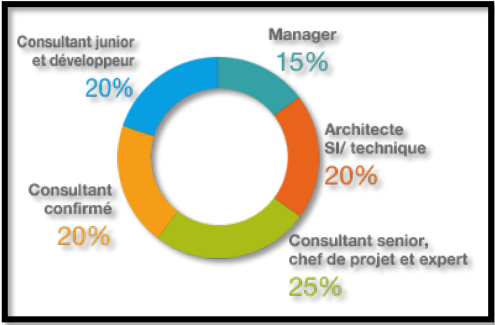
\includegraphics[scale=0.9]{neoxiaprofil.png}
\caption{Réputation de l'ffectif par profil}
\end{figure}
\subsubsection{Chiffre d'affaire}
Le graphe ci-dessous montre le chiffre d’affaires de NEOXIA en France et son évolution
soutenu

\begin{figure}[H]
\centering
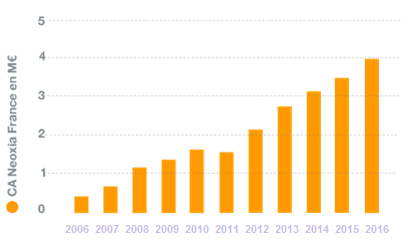
\includegraphics[scale=0.9]{ca.png}
\caption{Chiffre d'affaire NEOXIA France en Million d'Euros.}
\end{figure}
Le graphe ci-dessous montre le chiffre d'affaire de NEOXIA au Maroc et son évolution soutenue.
\begin{figure}[H]
\centering
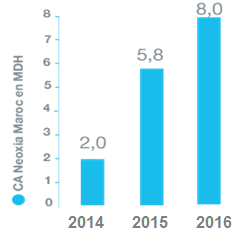
\includegraphics[scale=0.9]{nxmaroc.png}
\caption{Chiffre d'affaire NEOXIA Maroc en Million d'Euros.}
\end{figure}
Le graphe ci-dessous montre la répartition du chiffre d'affaire de NEOXIA par secteur
d'activités.
\begin{figure}[H]
\centering
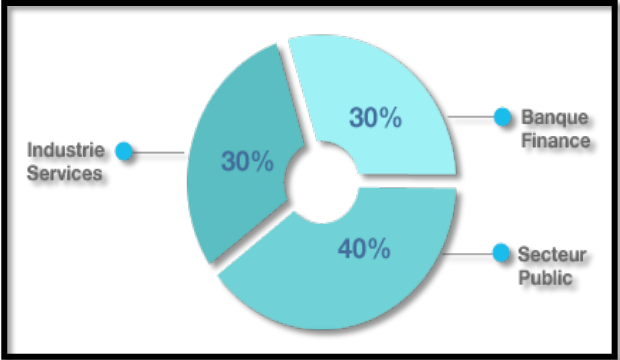
\includegraphics[scale=0.9]{secteur.png}
\caption{Chiffre d'affaire par secteur d'activités.}
\end{figure}

\subsection{Domaine de prédilection }
\subsubsection{Offre de service}
NEOXIA accompagne ses clients pour adresser les enjeux majeurs de leurs SI à différents
niveaux :
\begin{itemize}
	\item Stratégie et pilotage
- Schéma directeur et planification stratégique
- Architecture d'Entreprise
- Cartographie et Urbanisation
\item  Processus et organisation
- Management de projets et de portefeuille
- Audit et amélioration des processus
- Conduite de changement
- Management de la sécurité
\item  Conseil en architecture des SI
- Architecture orientée services et d’intégration
- Management de l’information
- Architecture logicielle et socles d’industrialisation
- Usine de développement et Socles technique
- Ateliers des tests logiciels
- Audit et refactoring du code
- Performance et sécurité IT
- Performance applicative et d'infrastructure
- Sécurité applicative et d’infrastructure
\item Infrastructure
- Architecture et revue d'infrastructure
- Cloud computing et Virtualisation
- Industrialisation de la gestion d'infrastructure
- Rationalisation des investissements d’infrastructure
\item  T ECHNOLOGIE ET SOLUTIONS
- Projets SI
- Assistance à maîtrise d’ouvrage
- Méthodologies agiles
- Coaching technique
- Développement d'applications
\item  Mobile
- Développement iPhone, Android, Black Berry
- Solutions mobiles
- Industrialisation du développement mobile
- SI entreprise mobile
\item Solutions
- Outils de management de projets
- Outils pour le management du SI
- Messagerie unifiée et collaboration
- Solutions SI métiers : Agricole, Mutuelle, Etablissements de formation
Pour assurer cet accompagnement, NEOXIA mène différentes typologies de missions :
\end{itemize}
\begin{itemize}
\item  Décider : Planification stratégique, Evaluation de maturité, Organisation, Audit,
Urbanisation, études, prototypage.
\item  Agir : Expertise, Développement et Intégration, Support, Coaching et Formation,
Accompagnement, Co-pilotage, Maîtrise des risques, Contrôle qualité .
\item  Capitaliser : Amélioration, Industrialisation, Réutilisation, Méthodes et bonnes
pratiques
\end{itemize}
\begin{figure}[H]
\centering
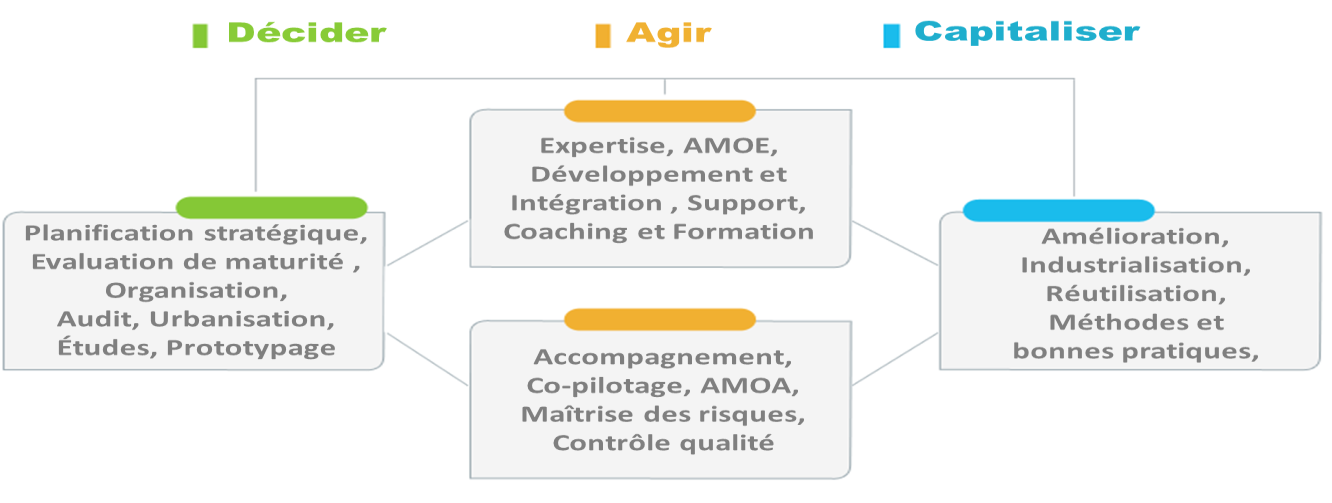
\includegraphics[scale=0.7]{dec.png}
\caption{les différentes typologies de mission de Neoxia.}
\end{figure}

\subsection{les principes de Neoxia}

Pour accompagner ses clients dans leur transformation digitale, 
Neoxia s'appuie sur plusieurs principes : 
\begin{itemize}
	\item \textbf{L'excellence } 
Sur chaque projet Neoxia se voit comme un partenaire. Elle s'engage sur des résultats concrets et des livrables clairs. 
\item \textbf{L'agilité}  
Neoxia prend soin d'appliquer le bon degré d'agilité en fonction du contexte client. Elle est membre fondateur de l'institut Agile & participant régulier du ScrumDay. 

	\item \textbf{La maîtrise des technologies } 
L'entreprise maîtrise un spectre large de technologie et veille à s'impliquer dans les nouvelles technologies émergentes.

\end{itemize}

\chapter{\textsc{Contexte du projet }}	 
Dans le cadre de sa stratégie destinée à intégrer les nouvelles technologies dans ses métiers et ses prestations, Neoxia Maroc, offre des services numériques et des solutions entreprises à ces clients alors qu'elle n'avait pas de Solution numérique pour gérer ses propres projets et ses affaires commerciales.

C'est dans ce cadre qu'intègre notre projet de fin d'étude, émanant du besoin d'une solution global répondant au fait de consolider toutes les données de l'entreprise dans une seule plateforme en restant branché à toute nouveauté à n'importe quel moment et de n'importe où.

\section{Presentation générale du projet}
\subsection {Déroulement du projet}
Le projet est passé par quatre phases importantes : 
\subsubsection {Documatation et formation}
	 Choix de la plateforme de développement :  Salesforce s'est avéré la meilleure solution à adopter pour développer une application web pour la gestion d'un processus commercial et accessible sur le Cloud.
 Nous avons suivi une   formation sur la plateforme de Salesforce nommée Trailhead : Trailhead permet d'accélérer la carrière en permettant d'acquérir ou d'approfondir les compétences Salesforce. Quel que soit le rôle (développeur, utilisateur, administrateur) ou le niveau (débutant ou expérimenté), Trailhead aide à comprendre grâce à ses différents parcours et modules, la plateforme applicative (App Cloud), le CRM (Sales Cloud) ou encore la plateforme analytique (Analytics Cloud). Les connaissances acquises sont certifiées au moyen de badges tout au long de l'apprentissage. Cet apprentissage se veut par ailleurs très pratique et concret puisque les badges s'obtiennent après une mise en pratique des connaissances acquises via de nombreux challenges (quizz, exercices...). Enfin, des projets concrets permettent d'appliquer son savoir dans des mises en situation aussi réalistes que possible (comme développer une application de gestion de conférences). Depuis son lancement, plus de 250 000 badges ont été attribués sur Trailhead. 
C'est dans ce contexte que nous avons fait notre formation sur la plateforme Salesforce. ou j'ai eu 61 badges, et 48625 points à la fin de la formation. 

\begin{figure}[H]
\centering
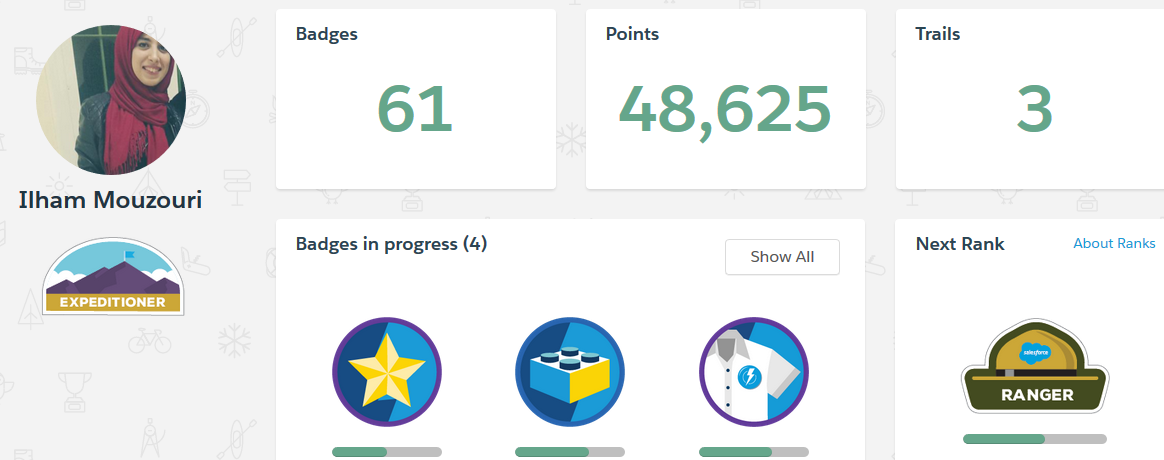
\includegraphics[scale=0.31]{rank.png}
\caption{Interface de la plateforme de formation TrailHead .}
\end{figure}
\subsubsection{	Conception } Nous avons fourni le data model adéquat pour l'application qui représente les différents objets standards et personnalisés à utiliser lors du développement de l'application. Ainsi l'élaboration de différents diagrammes selon les acteurs du système. 
\subsubsection { planification} 
La planification du projet est une phase importante d'avant-projet. Elle consiste à prévoir le déroulement de ce dernier tout au long des phases constituant le cycle de développement.
 Le diagramme de Gantt suivant présente le planning de mon projet :
\begin{figure}[H]
\centering
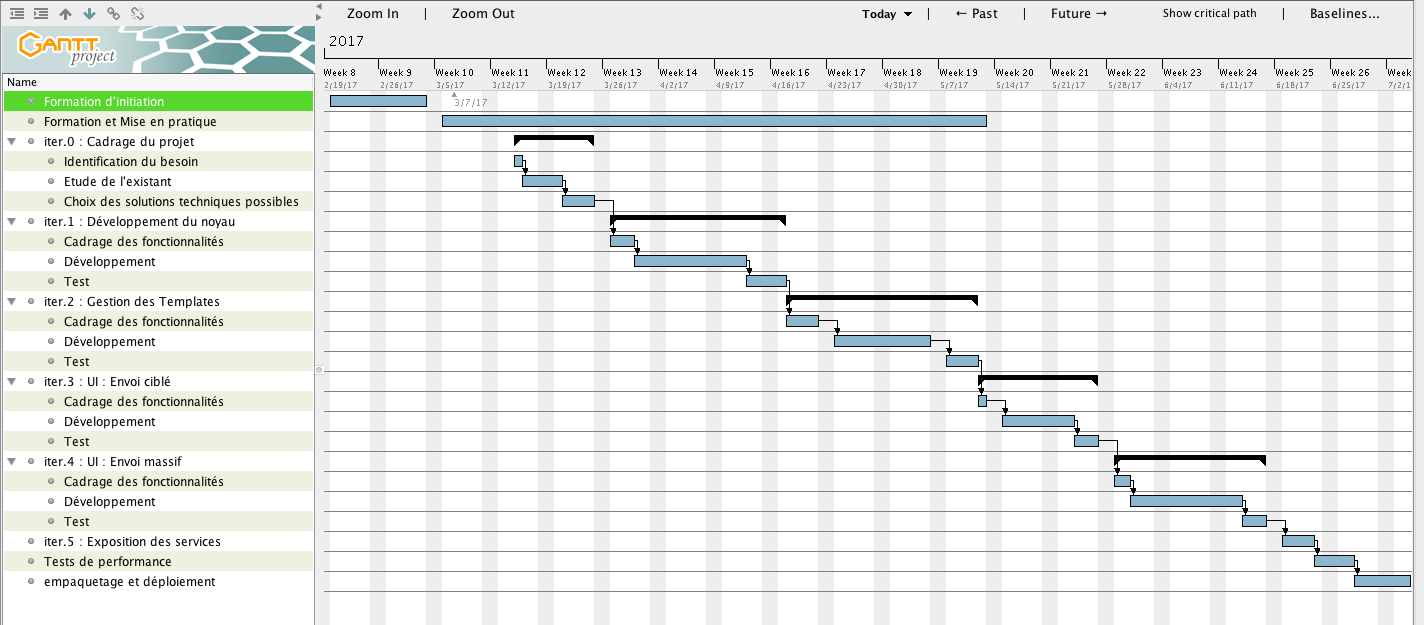
\includegraphics[scale=0.31]{gantt.png}
\caption{Diagramme de gant.}
\end{figure}

\subsubsection{	Réalisation} la réalisation était composé de plusieurs partie selon les processus détérminé pendant la phase de la conception initiale.  
\subsection{Conduite du projet}
\subsubsection{pratiques SCRUM}
La gestion de projet ou conduite de projet est une démarche visant à structurer, assurer et optimiser le bon déroulement d'un projet suffisamment complexe.Pour devoir réussir ce projet,
Il était nécessaire de se baser sur un cycle de développement sur lequel s'articule l'ensemble des solutions.
Ainsi Pour optimiser le temps disponible, nous avons travaillé en mode agile, c'est à dire en cycles itératifs courts permettant de fournir rapidement les fonctionnalités essentielles qui rendront l'application utilisable par les équipes.
Cette approche, inspirée de la méthode Scrum de développement informatique, permet de délivrer rapidement de la valeur métier.
Elle est particulièrement efficace dans les contextes où un retour utilisateur rapide est nécessaire.
 Une itération comprend trois étapes
\begin{itemize}
	
\item Planification de l'itération :
Chaque itération débute par une réunion avec l'encadrant (par exemple le lundi).
Lors de cette réunion, l'ensemble des fonctionnalités pressenties pour l'itération sont explicitées dans le détail, évaluées et priorisées.
\item	 Paramétrage et développements :
Les fonctionnalités sont ensuite implémentées et durant toute cette phase, le « contenu » de l'itération est fixe, mais des modification quotidiennes légères peuvent avoir lieu.
\item	Démonstration et validation :
A l'issue de l'itération on réalise une démonstration qui donne lieu à une validation ou à des modifications.
Cette réunion (par exemple le vendredi) est également l'occasion de faire une rapide rétrospective de l'itération (amélioration du fonctionnement) et de commencer à préparer la suivante.

\begin{figure}[H]
\centering
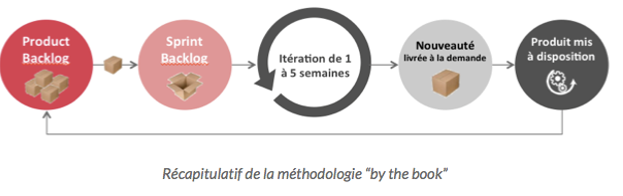
\includegraphics[scale=1]{Picture1.png}
\caption{le cycle de Scrum.}
\end{figure}
\subsubsection{Pratiques XP}
L'approche inspiré de SCRUM utilisé précedement, respecte plusieur aspect méthologique propre à la méthode SCRUM mais tous cela reste insuffisant pour mené un tel projet à la reussite , c'est pourquoi nous avons pensée à l'intégration de quelque pratique  de l'Extreme Programming  pour couvrir les techniques d'ingénierie logicielle.
\begin{itemize}
	\item 
\textbf{Cycles itératifs pilotés par le client :} Le projet progresse au rythme d'itérations très courtes, dont le contenu fonctionnel est déterminé par le client.
\item \textbf{Programmation pilotée par les tests :} On écrivait des test automatiques pour chaque portion de code qu'ils conçoivent, et on s'appui sur ces tests pour affiner et améliorer sans cesse la conception de l'application sans craindre de régression.
\end{itemize}
% -_-_-_-_-_-_-_ FIN Context General generale -_-_-_-_-_-_-_-_-_-_-_-_

% -_-_-_-_-_-_- CRM , Cloud Computing et Salesforce.com
 -_-_-_-_-_-_-_-_-_-_-_-_

\chapter{\textsc{Gestion des Relations Clients et Le Cloud Computing
}}

\section{La théorie de la Gestion des Relations Clients CRM }
Avant d’entamer la partie pratique de notre projet, il nous est paru judicieux de définir, dans un premier temps, la notion du CRM ou la Gestion des Relations Clients comme un ensemble de solutions technologiques spécialisées, permettant aux entreprises d’assurer un suivi de leur clientèle et de personnaliser leurs communications avec leurs marchés. Dans un deuxième temps, nous allons présenter le module SFA ou l’Automatisation des Forces de Vente puisqu’il est le module abordé durant notre projet. 
\subsection {Définition}
 Le CRM est un processus mettant en œuvre outils logiciels, méthodes, stratégie et comportements pour gérer plus efficacement la relation avec le client. Le processus commence dès l'étape de prospection des nouveaux clients et se poursuit en une recherche continue de fidélisation de clients à fort potentiel. D'une autre approche : C'est une méthode globale pour optimiser ses relations avec ses contacts (clients, prospects, prescripteurs...) afin d'avoir une meilleure connaissance de leurs besoins et d'y répondre le mieux possible ; tout en optimisant la rentabilité de cette relation. 
Il vise à proposer des solutions technologiques permettant de renforcer la communication entre l'entreprise et ses clients afin d'améliorer la relation avec la clientèle en automatisant les différentes composantes de la relation client :  
\begin{itemize}
	\item 
\textbf{L'avant-vente :} il s'agit du marketing, consistant à étudier le marché, c'est-à-dire les besoins des clients et à démarcher les prospects. L'analyse des informations collectées sur le client permet à l'entreprise de revoir sa gamme de produits afin de répondre plus précisément à ses attentes.  
\item	\textbf{ Les ventes :} L'automatisation des forces de vente (sales forces automation, SFA), consiste à fournir des outils de pilotage aux commerciaux afin de les assister dans leurs démarches de prospection (gestion des prises de contact, des rendez-vous, des relances, mais aussi aide à l'élaboration de propositions commerciales, ...). 
\item	\textbf{La gestion du service clientèle :} le client aime se sentir connu de l'entreprise et ne supporte pas devoir récapituler, à chaque prise de contact, l'historique de sa relation à l'entreprise. 
\item	 \textbf{L'après-vente :} consistant à fournir une assistance au client notamment via la mise en place de centre d'appel et via la mise en ligne d'informations de support technique. 
\end{itemize}
\subsection{les types du CRM}
Le CRM se présente sous trois variantes : 
\begin{itemize}
	\item 
	 \textbf{CRM opérationnel :} se charge de la gestion des forces de ventes, de l'organisation des campagnes, du service client.
C'est l’étape du CRM qui consiste à mettre en place la stratégie de gestion de la relation client qui a été adoptée par l'entreprise. Concrètement, le CRM opérationnel désigne la gestion de l'ensemble des canaux marketing, des flux d'information (en interface avec les données produites par et stockées sur l'ERP), des événements clients, des rythmes de travail et de toutes les actions de communication et de marketing conduites à l'intention du client. Son rôle est donc avant tout la coordination du FrontOffice avec le middle-office et le backoffice, et l'optimisation de leurs relations. Cela étend donc les activités traditionnelles du marketing à celles de la vente, a fortiori si l'entreprise est engagée dans un processus d'automatisation partielle ou totale de sa force de vente.
b.	 L'e-CRM : comprend notamment les techniques d'email marketing, les systèmes de personnalisation et de fidélisation en ligne et les outils de support client sur Internet. Avec leurs succès grandissants, les réseaux sociaux sont plus de plus intégrés aux outils e-CRM pour pouvoir en étendre leur portée : Les médias sociaux permettent d'engager les clients et les prospects. L'e-CRM permet d'échanger et partager avec ses clients, de créer une relation. Un moyen de les sonder, de les questionner, de prendre note de ce qu'ils disent et de réagir à leurs attentes. Il permet de construire une vue unique et centrale des clients et bâtir un profil de chacun d'entre eux. Avec l'e-CRM, il est possible de scénariser et d'automatiser les campagnes marketing. Détecter les clients les plus rentables et focaliser la stratégie marketing pour générer plus de revenus constitue est un des atouts de l'e-CRM. 
\item	CRM analytique : fournit une analyse statistique des données collectées, établit des ratios, donne les moyens d'analyser les performances de vente, les tendances, l'efficacité des campagnes ... 
C'est l'étape du CRM qui concerne la phase d'analyse de données collectées tout au long de la gestion de la relation client. C'est la phase pendant laquelle on va exploiter les informations sur le client et son comportement d'achat, afin de mieux le comprendre et donc si possible de l'anticiper à l'avenir à l'aide de modèles éventuellement. Souvent placé au cœur de la business intelligence de l'entreprise, le CRM analytique contribue à faciliter la prise de décision (établissement de typologies, définition de critères de segmentation, recommandation pour la capitalisation en termes d'image, structuration et évolution des gammes de produits et de services…).
\end{itemize}
\subsection{Les fonctionnalités du CRM }
Le CRM ou la gestion de la relation client consiste à identifier, à retenir et à développer les clients les plus profitables et en acquérir des nouveaux. C'est une stratégie d'entreprise orientée vers la satisfaction et la fidélité du client, elle est axée sur le marketing différencié, personnalisé ou One to One. Il repose sur deux principes : 
a.	Tous les clients ne sont pas égaux. 
b.	Le comportement suit la promesse de la récompense. 
Les fonctions d'un CRM peuvent être résumé à : connaître, choisir, conquérir et fidéliser la clientèle.  
  
\begin{enumerate}
	\item 
	\textbf{Connaître le client :} l'entreprise doit rassembler les informations lui permettant de décrire et de caractériser sa clientèle, de la positionner sur son marché et de détecter de nouveaux segments. 
Tous les moyens technologiques existent aujourd'hui pour constituer, gérer et analyser des quantités massives de données. Gérer la relation client consiste à valoriser son capital client. D'un point de vue technique, le CRM implique de capturer, au niveau de l'entreprise, l'ensemble des données clients, collectées en interne ou auprès d'organisations extérieures, et de les intégrer dans un Data Warehouse (entrepôt de données) orienté client. 
\item	\textbf{Choisir son client :} l'étape suivante consiste à analyser ces données avec les techniques les plus évoluées. Le Datamining, analyse statistique et à rendre les résultats accessibles à tous les canaux d'interaction avec les clients. Le Datamining permet d'analyser et d'interpréter un gros volume de données, de différentes sources afin de dégager des tendances, de rassembler les éléments similaires en catégories statistiques et de formuler des hypothèses. A partir des informations collectées, l'entreprise pourra obtenir des réponses objectives sur lesquelles fonder sa stratégie opérationnelle. La centralisation des données clients doit ainsi faciliter le pilotage de toute l'activité de la société. En effet, l'informatique décisionnelle (Business Intelligence et Datamining) permet d'élaborer les diverses composantes de la stratégie : (commerciale, marketing, canaux de vente, fidélisation) et fournit tous les tableaux de bord nécessaires. Ainsi il faut différencier les clients en fonction de leur besoin et de leur contribution au résultat et dialoguer avec eux de manière à diminuer les coûts de la relation commerciale et à en augmenter l'efficacité. Ce dialogue doit permettre de faire remonter l'information. 
\item	 \textbf{Conquérir de nouveau client :} la mise en œuvre d'une stratégie orientée client concerne l'ensemble du processus commercial. Les nouveaux canaux de ventes (télévente, commerce électronique, etc.) créent des opportunités métiers. De nouveaux outils (Sales Forces Automation) permettent aux commerciaux de mieux gérer leur activité et d'augmenter leur efficacité en construisant leurs propositions en interaction directe avec le client. 
\item	\textbf{Fidéliser les meilleurs clients :} Les programmes de fidélisation bénéficient de nouvelles possibilités technologiques, telle que la carte à mémoire. Le service après-vente devient l'occasion privilégiée de concrétiser une relation personnalisée et durable avec le client, en lui proposant une offre encore mieux adaptée à ses besoins.
\end{enumerate}

\section{Cloud Computing}
\paragraph{}
Le Cloud Computing, ou informatique en nuage, est, outre ses nouvelles
spécificités techniques, un nouveau concept. Cette nouvelle façon de penser et de
concevoir le rapport homme/machine s'inscrit dans un cycle bien plus large : pendantlongtemps la machine n'était qu'une simple interface de visualisation de l'information et tout son traitement était internalisé (l'ère du Minitel), puis les machines ont
embarqué de la puissance de calcul et de la mémoire et les calculs ont alors été externalisés et effectués en local. La « course à la puissance » était engagée jusqu'à la saturation de la fréquence de l'horloge interne de l'ordinateur. Aujourd'hui, nous nous dirigeons, avec l'émergence des tablettes tactiles, vers un retour à la notion d'interface de travail. Logiciels et données sont dans la majeure partie hébergés dans des serveurs privés ou communautaires à travers le monde.
Ce nouveau concept, qui se traduit dans la réalité économique par une restructuration inévitable de la filière informatique comme nous le verrons par la suite, consiste à fournir des capacités de traitement informatique évolutives, élastiques et mises à disposition comme un service pour les utilisateurs qui y accèdent via internet sans gestion de l'infrastructure sous-jacente. La notion d'évolutivité et d'élasticité s'explique par le fait que l'utilisateur peut faire varier les ressources demandées à la
hausse comme à la baisse et ce de manière très dynamique, avec une facturation des ressources à la consommation. Les capacités informatiques concernées par le Cloud Computing sont variées : capacité de calcul, espace de stockage, bande passante ou
encore logiciels.
Les applications proposées en mode Cloud Computing ne se trouvent plus forcément sur un serveur informatique hébergé chez l'utilisateur mais dans un « nuage» formé de l'interconnexion de serveurs géographiquement distincts réalisée au niveau
de fermes de serveurs géantes (également appelées Datacenters). Ceci est rendu possible par le procédé de virtualisation qui consiste à faire fonctionner plusieurs systèmes d'exploitation ainsi que leurs applications associées sur un seul serveur
physique. La virtualisation permet ainsi de recréer plusieurs ordinateurs virtuels sur une seule et même machine physique.

\subsection{Apports techniques du cloud computing }
	
Parmi les apports techniques du cloud, on trouve : 
 
\begin{itemize}
	\item 
	Automatisation – « l'infrastructure scriptable » : Nous pouvons mettre en place des processus reproductibles de construction (build) et de déploiement applicatif, et ceci en pilotant l'infrastructure via une interface de programmation. 
 
\item	Adaptation automatique de la capacité (auto-scaling) : Nous pouvons adapter la capacité en fonction du besoin de vos applications, que ce soit pour la réduire ou pour l'augmenter, et ceci sans intervention humaine. L'auto-scaling facilite l'automatisation, et amène d'avantage d'efficacité. 
 
\item	Adaptation proactive de la capacité (proactive scaling) : Nous pouvons également anticiper, en planifiant à l'avance la capacité en fonction de la fréquentation attendue. 
 
\item Cycle de développement plus efficace : Les environnements de production peuvent être aisément dupliqués pour fournir les environnements de développement, de test, et de préproduction. Les environnements préproduction peuvent aisément passer au stade de la production. 
 
\item	Amélioration de la testabilité : Pour le test, Nous ne sommes jamais à court de hardware. Nous pouvons introduire les tests et les automatiser à tous les stades du processus de développement. Pour une campagne de test, nous pouvons quasi-instantanément dériver un environnement de test préconfiguré, et le supprimer en fin de campagne. 
 
\item	Plans de reprise et de continuité d'activité facilités : Le cloud permet une approche plus efficace du plan de reprise d'activité et du plan de continuité d'activité, en permettant de disposer des serveurs et du stockage de données à moindre coût. Nous pouvons répartir nos infrastructures sur de multiples sites géographiques. Nous pouvons dupliquer un environnement complet sur un autre site en quelques minutes. 
 
\item	Utilisation du cloud comme "trop-plein" : Quelques clics et une politique de load balancing adaptée permettent de déverser le trop-plein de fréquentation d'une application vers le cloud.
\end{itemize}

\subsection{	Apports économiques du cloud computing }
Construire des applications pour le cloud présente des avantages certains sur le plan économique. Voici quelques-uns de ces avantages. 
\begin{itemize}
	\item 	Suppression quasi-totale des investissements amont d'infrastructure : Construire des systèmes de grande capacité nécessite des investissements très importants en surface de locaux, en sécurité physique, en hardware (racks, serveurs ; routeurs, alimentation de secours), en fonctionnement de hardware (coûts énergétiques et climatisation), et en personnel. De part leur ampleur, ces coûts doivent être anticipés en amont et mettent en œuvre un processus décisionnel long et complexe, et ceci avant même que le projet ne puisse démarrer. Avec le cloud, de tels frais fixes ou de démarrage n'existent plus. 
 
\item	Infrastructure à la demande : Auparavant, si votre application attirait les utilisateurs en nombre et que le l'application ou l'infrastructure n'était pas capable de faire face, vous vous retrouviez victime de votre propre succès. Ou alors, si vous aviez investi lourdement et que les utilisateurs ne venaient pas aussi nombreux qu'espérer, vous étiez cette fois victime de votre échec. Déployées sur le cloud, les applications bénéficient d'un dimensionnement à la demande de l'infrastructure. Il n'est plus nécessaire de recourir à l'acquisition anticipée de capacité d'infrastructure. Vous augmentez la capacité au fur et à mesure de vos besoins, et payez uniquement ce que vous utilisez vraiment. La flexibilité s'en trouve augmentée, et les risques et les coûts d'exploitation, réduits. 
 
\item Utilisation plus efficace des ressources : Les administrateurs système sont habituellement préoccupés par l'acquisition de hardware supplémentaire (quand la capacité est insuffisante) ou par le désir de mieux utiliser la capacité disponible (en cas d'excès de capacité ou de capacité inexploitée). Avec le cloud, ils peuvent utiliser les ressources plus efficacement, en laissant l'application demander et restituer elle-même les ressources selon ses besoins. 
 
\item Coûts modulés selon l'usage : Avec une tarification au service, vous êtes facturé uniquement pour l'infrastructure que vous utilisez. Vous ne payez pas pour de l'infrastructure qui vous est affectée, mais que vous n'utilisez pas. Ceci fait apparaître une nouvelle perspective de réduction des coûts. Ainsi, quand vous déployez un correctif d'optimisation des performances, vous constatez une réduction quasi-immédiate de vos coûts (parfois dès la fin du premier mois). Par exemple, dans le cas où l'introduction d'un cache permet de réduire de 70 \% 
les requêtes de données, les économies réalisées démarrent immédiatement et continuent de s'accumuler avec le temps ; la récompense ne tarde pas à tomber dès la facture suivante. De plus, si vous construisez une plateforme fondée sur le cloud, vous pouvez propager le mode de tarification modulé par l'usage à vos propres clients. 
 
	\item La réduction des délais de livraison : La parallélisation est l'un des moyens les plus efficaces pour accélérer la vitesse de traitement. Si un traitement lourd, mais parallélisable, dure 500 heures sur une seule machine, avec les architectures cloud, il est possible de répartir ce traitement sur 500 instances, réduisant ainsi son exécution à 1 heure. Disposer d'une telle infrastructure 'élastique' permet à l'application de mettre à profit la parallélisation, et de réduire pour le métier le délai de mise à disposition du résultat. 
\end{itemize}
\chapter{Analyse Fonctionnelle et Conception}
Ce chapitre présente une étude détaillée des spécifications fonctionnelles du projet. La première section traite les besoins fonctionnels et non fonctionnels du projet visant à reformuler le besoin d'une manière simple et réalisable. La deuxième section est une analyse des acteurs qui interviennent dans le projet. Quant à la troisième, il s'agit d'une modélisation pour donner une vision globale du comportement fonctionnel de notre solution. 
\section{ Spécifications fonctionnelles }
\paragraph{}
Les spécifications fonctionnelles générales de l'application ont été décrites en collaboration avec l'encadrant, et le client qui est en fait le directeur Général de Neoxia au Maroc et l'assistante chargé de facturation. Des plans d'action élaborés pendant les réunions précisaient le périmètre général ainsi que les différentes fonctionnalités que l'application devrait offrir. Une fois ayant procédé à une analyse détaillée, nous avons pu identifier les différentes exigences métiers. 
Le besoin de Neoxia à gérer ses propres affaires sur une plateforme Salesforce, m'a amené à comprendre le métier de gestion des projets informatique ainsi que la gestion des prestations.
Ensuite comprendre le déroulement des ventes des prestations dès la phase de marketing allant à la phase du SAV.
Le processus global se compose de plusieurs sous-processus
\begin{enumerate}
	\item {	Processus de Marketing}
	Après avoir organisé des actions publicitaires et accueillir un nombre important de pistes, comptes, contacts et opportunités.
L'entreprise commence la phase du marketing pour pouvoir commencer ses affaires et vendre ses produits.
La tendance du marketing nous mène directement vers le mass mailing.
L'utilisateur doit être capable d'envoyer des e-mails en mass aux contacts et pistes enregistrés sur la plateforme avec des modèles bien précis pour chaque cas,  de nos jours le consommateur recherche des aspects comme le plaisir, la sécurité, la considération, et surtout la personnalisation. Ces nouveaux critères obligent les entreprises à mettre en place les processus nécessaires à la rencontre de ces attentes.
C'est pourquoi les modèles des e-mails sont divers et personnalisés.
Mais le processus ne s'arrête pas là, car le client va répondre par une demande, réclamation ou juste une question, on doit être capable de capturer la réponse, la stocker et par la suite crée une tâche pour pouvoir traiter la demande.
Après l'exécution de la tâche elle est marquée comme terminée. 

La figure ci-dessous représente le processus de marketing.
\begin{figure}[H]
\centering
\caption{Diagramme des cas d'utilisation}
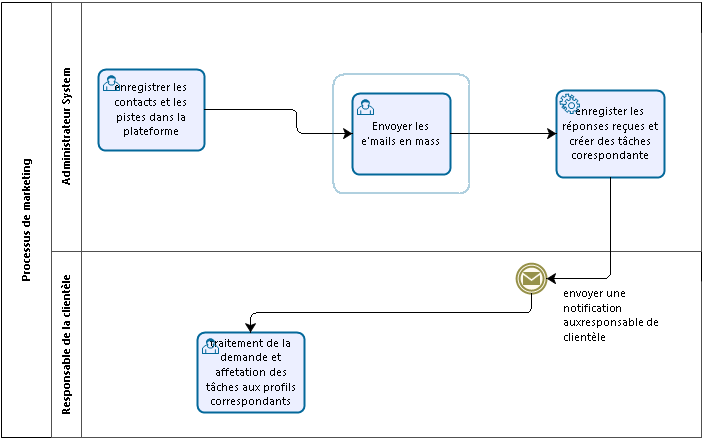
\includegraphics[scale=0.41]{processusmarketing.png}
\end {figure}
\item{Processus de ventes }
Le processus de vente commence par la création d'une piste, par la suite cette piste est soit supprimée si elle n'est pas qualifiée, soit qualifiée et convertie.
Une piste convertie nous donne un Compte, Contact et Opportunité.
Une fois nous avons notre opportunité ouverte dans l'org, on commence à concentrer sur l'objet Opportunité qui passe par plusieurs étapes selon l'évolution des propositions et des échanges avec le client :
La figure si dessous montre le déroulement du processus de vente.
\begin{figure}[H]
\centering
\caption{Schéma du processus de vente.}
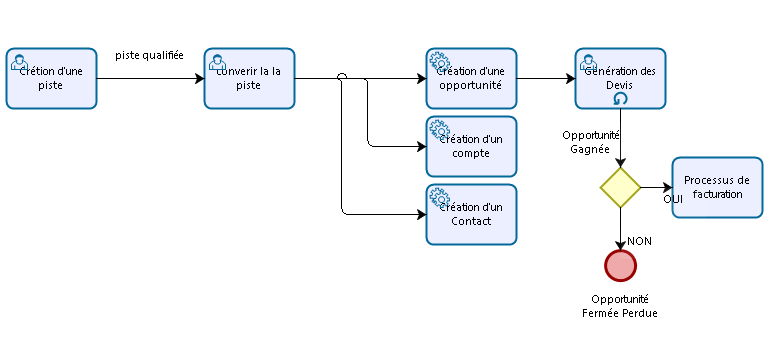
\includegraphics[scale=0.75]{processusvente2.png}
\end{figure}
L'objet opportunité passe par des étapes claire et nette sont :
	
	\begin{itemize}
		\item Prospection 
		\item Qualification
		\item Proposition des valeurs
		\item Offres Commerciale
		\item Négociation
		\item Fermée gagnée/Perdue.
\end{itemize}
C'est dans la phase de l'offre commerciale que commence l'envoi des Devis, jusqu'à l'acceptation d'un devis de la part du client, et là on dit que l'opportunité est gagnée. Et on commence le processus de facturation.

\item {Le processus de facturation }
Ce processus est déclenché par l'acceptation du devis par le client, cette acceptation envoie automatiquement une notification au Responsable commercial pour qu'il crée des tâches pour chaque date de facturation, quand la date est échue le responsable de facturation est notifié, qui va par la suite demandé au Responsable Commercial de lui confirmer la validation de la réception pour que le responsable de Facturation Dépose la facture sinon la  date de dépôt est modifié.
Ensuite après le dépôt de la facture si la facture est réglée dans le délai, elle est marquée comme réglée. Sinon une relance sur le règlement est lancée par le Responsable du Recouvrement.

\begin{figure}[H]
\centering
\caption{Processus de facturation}
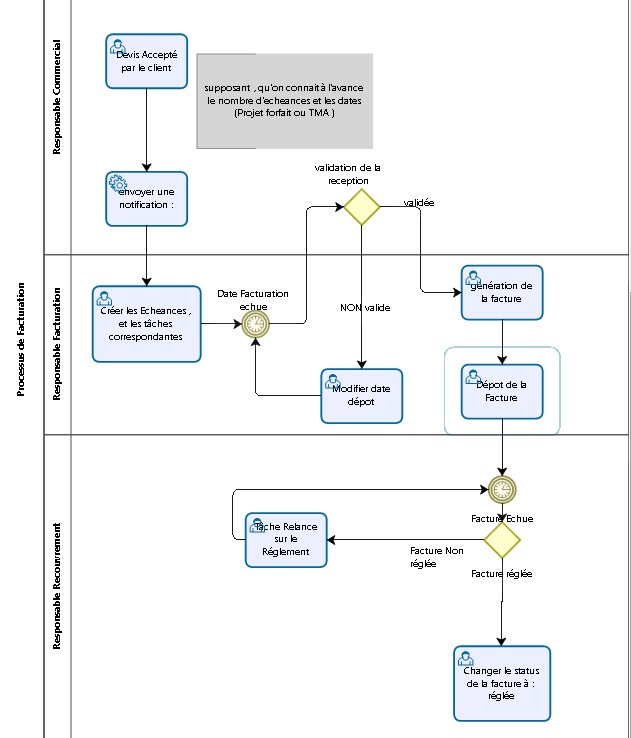
\includegraphics[scale=0.9]{processusfacturation.png}
\end{figure}
\item {Lightning Sync}
Google a maintenant des fonctions de calendrier. La synchronisation du calendrier de salesforce avec le calendrier Google nous permettrait de fournir des tâches à un ensemble diversifié d'outils utilisés dans le domaine. Comme les téléphones cellulaires ... Cela permettrait aux clients de numériser des calendriers de vente pour réserver l'heure et nous pourrions lier cela à Salesforce. Le calendrier Google peut être mis à jour depuis le téléphone portable ( depuis l'Agenda de Google). 
cette figure montre le résultat final de cette configuration dans Google Contacts:
\begin{figure}[H]
	\centering
		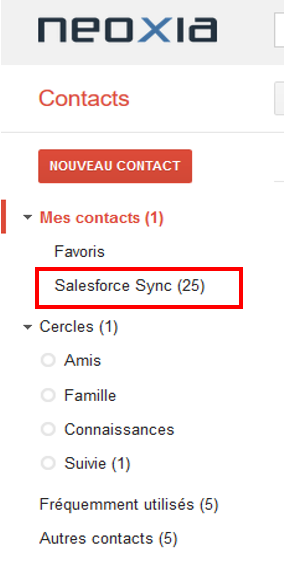
\includegraphics{Contactsync.PNG}
	\label{fig:les Contacts Synchronisés de SF vers Google Contacts}
\end{figure}
 




\end{enumerate}

\section{Conception}
Toute personne qui utilise une base de données relationnelle sait que la structure de stockage de base de données primaire est une table, une structure de données qui possède un ensemble de champs (colonnes) avec des types de données spécifiques comme texte, date et numéro. Les applications gèrent les informations des tables par la création, la lecture, la modification et la suppression des enregistrements (lignes).

Avec Force.com, la première structure de données est appelée un objet, qui, avec quelques fonctions supplémentaires, est plus ou moins le même concept que la table, mais nous avons que deux types de relation entre les tables :
	
	\begin{itemize}
		\item Relation Principal-détails : Master-détail.
		\item Relation de référence : lookup.
\end{itemize}
Les relation « principal-détails » et « de référence » facilite l'association entre les objets, Il n'est pas nécessaire de déclarer les clés primaires et étrangères, et compliquer la structure avec les jointures.
la figure ci-dessous représente le schéma généré par Salesforce  qui schématise quelques objets crées dans l'org.
\begin{figure}[H]
\centering
\caption{la clé du générateur de schéma}
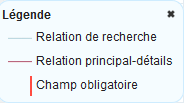
\includegraphics[scale=1]{key.png}
\end{figure}
\begin{figure}[H]
\centering
\caption{le schéma des Objets utilisés dans l'org}
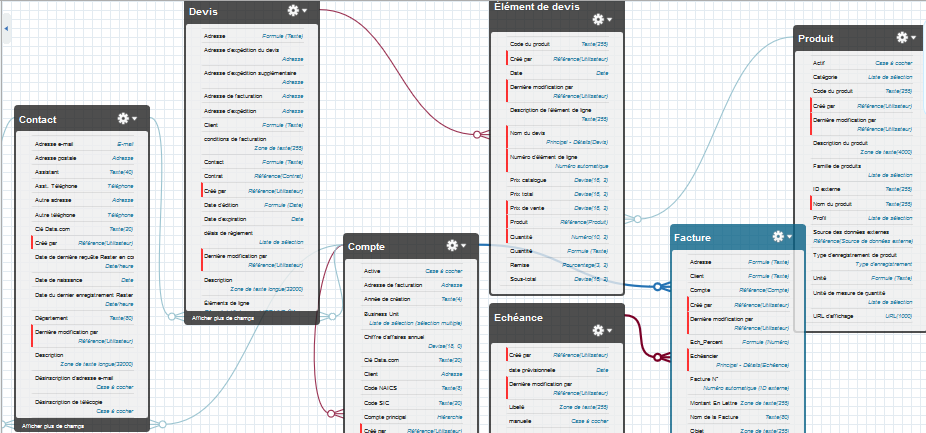
\includegraphics[scale=0.6]{schemabuilder.png}
\end{figure}


 
% -_-_-_-_-_-_-_-_-_-_-_-_ Etude technique  -_-_-_-_-_-_-_-_-_-_-_-_

\chapter{\textsc{Étude technique}}

\paragraph{}
Dans ce qui suit, le plan technique du projet sera abordé. On présentera ainsi les contraintes techniques liées aux outils de développement utilisés durant la réalisation du projet. L'architecture physique et applicative seront détaillées pour avoir une vision claire sur la démarche de mise en oeuvre de la solution. 


\paragraph{}
Salesforce.com est un éditeur de logiciels, basé à San Francisco aux États-Unis. Il distribue des logiciels de gestion basés sur Internet et héberge des solutions pour la gestion de la relation client CRM.
Précurseur du Cloud Computing, et aujourd'hui leader mondial des outils CRM, Salesforce compte plus de 100 000 entreprises clientes dont Pernod Ricard, Renault, Cofely GDF SUEZ ou encore IBM.

\subsubsection{Produits et services \textsc{salesforce.com} : }

 \paragraph{}
Basé sur Database.com et un marché d'applications d'entreprise Appexchange, les solutions de Salesforce.com sont regroupées sous plusieurs grandes catégories : 

\begin{figure}[H]
\centering
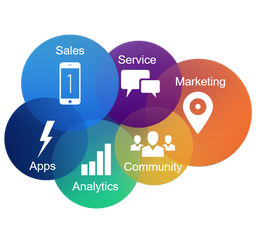
\includegraphics[scale=2]{clouds.png}
\caption{Les services SalesForce en Cloud.}
\end{figure}

\begin{description}

\item{\textit{Sales : }}

	\begin{itemize}
		\item \textbf{Sales Cloud : } automatisation des processus de vente et CRM.
		\item \textbf{Data.com : } prospection B2B et nettoyage de données.
	\end{itemize}
	
\item{\textit{Service : }}

	\begin{itemize}
		\item \textbf{Service Cloud : } service d'assistance entièrement personnalisable.
		\item \textbf{Desk.com : } service d'assistance clientèle pour les petites entreprises.
	\end{itemize}
	
\item{\textit{Marketing : }}

	\begin{itemize}
		\item \textbf{Marketing Cloud : } plate-forme de marketing numérique.
		\item \textbf{Pardot : } automatisation des processus Marketing B2B.
	\end{itemize}
	
\item{\textit{Community : }}

	\begin{itemize}
		\item \textbf{Community Cloud : } communauté des clients,  partenaires et employés.
		\item \textbf{Chatter : } réseau social d'entreprise.
	\end{itemize}
	
\item{\textit{Analytics : }}

	\begin{itemize}
		\item \textbf{Wave Analytics : } business Analytics sur toute donnée et tout périphérique.
		\item \textbf{Wave Apps : } des applications qui influencent l'attrait des ventes et le plaisir des clients.
	\end{itemize}
	
	
\item{\textit{Platform and Apps : }}

	\begin{itemize}
		\item \textbf{Salesforce1 : } La plate-forme du Cloud développement n ° 1 .
		\item \textbf{Force.com : } Automatisation des processus métier moyenant des applications.
		\item \textbf{Heroku : } Création d'applications orientées client.
	\end{itemize}
	
\item{\textit{Marketplace : }} Achat et vente d' applications

\end{description}

\paragraph{}
\textsc{salesforce.com} offre une panoplie d'outils standards intégrés permettant l'automatisation des processus et le stockage des données d'une entreprise. En revanche, et lorsqu'une fonctionnalité n'est pas intégrée par défaut dans la solution, La plate-forme offre aux développeurs des outils puissants pour développer leurs propres nouvelles fonctionnalités, et ce, avec une complète compatibilité (aussi logique qu'esthétique) avec ce qui existe par défaut. 
\subsection {MVC et Salesforce}
Le paradigme Modèle, Vue et Contrôleur
\begin{figure}[H]
	\centering
		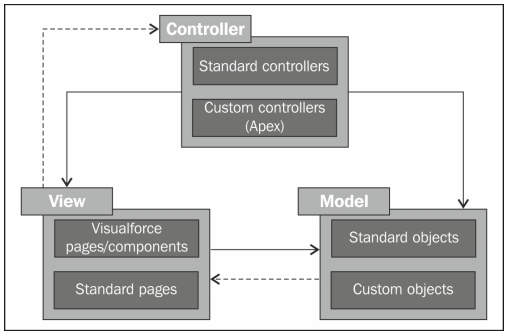
\includegraphics{mvc.png}
	\label{fig:MVC en Salesforce}
\end{figure}
\paragraph{}
Comme illustré sur la figure ci-dessus, Model View Controller (MVC) est un
patron de conception qui sépare la couche de présentation de la couche métier qui
interagit avec l'utilisateur. En plus de la séparation de l'application en trois couches,
le patron MVC définit les interactions entre ces différentes couches
\paragraph{}Ce patron de Salesforce contient donc trois modules suivants :
\begin{itemize}
	\item {Modèle :} Traitements des données, interactions avec la base de données dans
Salesforce. Ainsi les objets standards et personnalisés, différents champs et relations font partie de cette couche.`
\item{Vue :} la façon dont les schémas et les données sont représentés. Les pages
Visualforce, pages Layout et les différents onglets déterminent la couche Vue
du MVC
\item{Contrôleur :} Les contrôleurs sont utilisés afin d'exécuter les actions de l'interaction de l'utilisateur avec Visualforce, et ce module est définit par les
Workflows, Apex Classes et Triggers.
\end{itemize}

\paragraph{SFDC\foornotemark[1] MVC }
on peux écrire les pages "`VUE" en utilisant SFDC visual force (VF). les pages VF sont similaires aux pages JSP.chaque page VF est associée à un Controlleur.soit on utilise les Controlleurs Standard ou écrire nos propre controlleurs en utlisant le language Apex. 
\paragraph{}
Visualforce utilise le paradigme traditionnel : Modele-vue-controlleur,avec l'option d'auto-générer les controlleurs pour les objets de la base de données,Fournissant une intégration complète et simple avec la base de données. Vous pouvez écrire vos propres contrôleurs, ou des extensions aux contrôleurs, en utilisant le code Apex. Visualforce fournit également des composants ajax et inclut le langage d'expression de formule pour l'interaction d'action, de données et de liaison de composants.
\paragraph{}
SFDC MVC pattern contient les modules suivants 
\begin{enumerate}
	\item Modèle 
	\item vue
	\item Controlleur
\end{enumerate}
\paragraph{Modèle}
le modèle et le schéma et les données qu'utilise salesforce pour représenter le système complèt. Dans SF on peut dire que \textbf{sObjects}sont le modèle, comme toute entité dans SF est mappée avec un sObject.
\paragraph{Vue}
est comment le schéma et les données sont représentées. VisualForce est utilisé pour présenter les données aux utilisateurs.
\paragraph{Controlleur}
comment les intérface se comportent. les controlleurs sont utilisés pour. Les contrôleurs sont utilisés pour effectuer les actions chaque fois que les utilisateurs interagissent avec le visualforce

Salesforce.com est un outil primé pour gérer toutes les données de l'équipe commerciale d'une organisation. La flexibilité et l'assurance des données sécurisées fournies par Salesforce.com entraînent des capacités de développement non parallèles pour le développeur
 
\section {Les objets Standard de Salesforce}

\section{Exigences techniques}

\subsection{La PAAS\up{1} \textsc{salesforce.com}}
\footnotetext[1]
{Platform as a Service, souvent appelé simplement PaaS, est une catégorie de services de Cloud computing qui fournit la plateforme et l'environnement informatique nécessaire aux développeurs pour mettre en place leurs différents services et applications sur Internet.}
\paragraph{}
SALESFORCE est une plate-forme hautement personnalisée. En plus de la multitude des fonctionnalités offertes pour les utilisateurs de la plate-forme, cette dernière permet d'étendre ses fonctionnalités standard, créer des pages, des composants et des applications entièrement personnalisées.
\paragraph{}
Le développement dans la plate-forme SALESFORCE garantit les avantages suivants : 
\begin{description}
\item{\textbf{Sécurité : }} SALESFORCE offre à ses utilisateurs un contrôle total et précis de la sécurité de toute activité. Depuis l'authentification des utilisateurs, les autorisations administratives d'accès aux données jusqu'au modèle de partage. 
\item{\textbf{Mutualisation : }} Le fait que les ressources informatiques dans un contexte de Cloud sont dématérialisées, les rend accessibles à tous les utilisateurs. Ces ressources sont partagées pour éviter à des utilisateurs d'investir dans des ressources sous risque d'une sous-exploitation dans les périodes moins actives.
\item{\textbf{Gain de temps : }} Dans un cas normal, la mise en oeuvre d'une application a besoin du matériel et du logiciel, une configuration d'accès et de sécurité seront obligatoires et des rapports doivent être configurés. Avec SALESFORCE aucun logiciel n'est matériel n'est installé par le développeur. En effet, on peut définir ses propres configurations de sécurité des données, créer des rapport et rendre son application sociable et mobile.  
\item{\textbf{Scalabilité : }} les données et métadonnées sont activés via des API. Cela signifie qu'ils sont accèssibles depuis un point unique et exploitables partout. 
\end{description}

\subsection{Outils utilisés}
\paragraph{}
Du moment que le développement sera sur une plate-forme hébergée en Cloud, les outils et langages utilisés seront imposés par la plate-forme même.
\subsubsection{APEX}
\begin{figure}
	\centering
		
\includegraphics[scale=0.5]{SalesforceApex.png}
	\label{fig:logo Apex}
\end{figure}

Le premier langage de programmation à la demande\footnotemark[2] au monde. Apex Code étend le succès puissant et éprouvé de la plate-forme \textsc{Force.com}\footnotemark[3] en introduisant la possibilité d'écrire un code qui s'exécute sur les serveurs \textsc{salesforce.com}. La langue permet de développer et de déployer entièrement une nouvelle classe d'applications et de fonctionnalités à la demande. Ces applications rendent les applications existantes de \textsc{Force.com} «plus intelligentes» en leur permettant de capturer la logique métier et les règles - telles que la validation des données - et développer des applications entièrement nouvelles à la demande - telles que la vérification complexe des stocks et l'exécution des commandes.

\footnotetext[2]{Les languages à la demande sont fournis par un fournisseur de services, et ont la particularité d'être compilés et exécutés dans le cloud, sont facilement distribués et ne nécessitent généralement pas de logiciels que ce qui est standard avec la plupart des systèmes d'exploitation.}

\footnotetext[3]{Force.com est une plate-forme de développement d'applications sociales et mobiles de Salesforce.com.}


\subsubsection{VISUALFORCE}
\begin{figure}[H]
	\centering
		
\includegraphics{Visualforce.jpg}
	\label{fig:Visualforce}
\end{figure}

\paragraph{}
Visualforce est un Framework qui permet aux développeurs de créer des interfaces utilisateur sophistiquées et personnalisées qui peuvent être hébergées en mode natif sur la plate-forme Force.com. Il inclut un langage de balisage similaire à HTML.
Dans le langage de balisage Visualforce, chaque étiquette VF correspond à un composant d'interface utilisateur grossier ou à grains fins, comme une section d'une page, une liste de sélection ou un simple champ. 
\paragraph{}
Le comportement des composants Visualforce peut être commandé par la même logique qui est utilisée dans les pages Salesforce standard ou par une logique spécifique écrite dans Apex comme un controlleur personnalisé.

\subsubsection{SOQL : Salesforce Object Query Language}

\paragraph{}
SOQL est un langage informatique propriétaire à Salesforce servant à effectuer des opérations sur des objets Salesforce. Il est utilisé pour construire des chaînes de requêtes simples mais puissantes dans les environnements suivants:
\begin{itemize}
\item	Dans des déclarations Apex ;
\item	Dans les contrôleurs Visualforce ;
\item	Dans l'Explorateur de schéma de l'IDE Force.com.
\end{itemize}
\paragraph{}
Sa syntaxe est similaire à celui de SQL (Structured Query Language), Il permet de spécifier l'objet source, une liste des champs à récupérer, et les conditions de sélection des lignes dans l'objet source.

\subsubsection{JAVASCRIPT}
\begin{figure}[H]
	\centering
		
\includegraphics{js.png}
	\label{fig:js}
\end{figure}

\paragraph{}
JavaScript est un langage informatique utilisé sur les pages web. Ce langage a la particularité de s'executer sur le poste client. En effet, le client reçoit le code dans son navigateur puis l'exécute.
JavaScript n'a aucun rapport avec le Java qui est un autre langage informatique.
\paragraph{}
La particularité du JavaScript consiste à créer des petits scripts sur une page HTML - ou VISUALFORCE dans mon cas - dans le but d'ajouter une petite animation ou un effet particulier sur la page. Cela permet en général d'améliorer l'ergonomie ou l'interface utilisateur. L'intérêt du JavaScript est d'exécuté un code sans avoir à recharger une nouvelle fois la page.

% -_-_-_-_-_-_-_-_-_-_-_-_ FIN Etude technique  

% -_-_-_-_-_-_-_-_-_-_-_-_ Realisation  -_-_-_-_-_-_-_-_-_-_-_-_

\chapter{\textsc{Mise en oeuvre}}
\section{développement du processus de vente}
\subsection{Identification des Objets}
Tous d'abord nous avons fait une conception initiale pour les objets utilisés dans ce processus, qui nous a permis de tirer les objets suivants :
Piste , Compte , Contact, Opportunité Devis et Elements de Devis
la figure ci-dessous schématise les objets nécessaires pour la création de ce processus:
\begin{figure}[H]
	\centering
		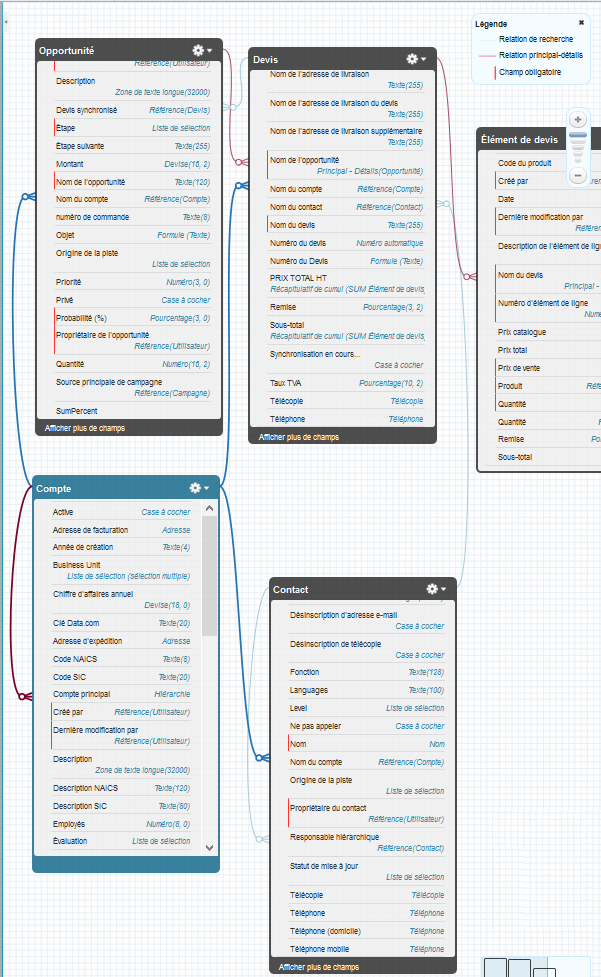
\includegraphics{classvente.PNG}
	\label{fig:classvente}
\end{figure}
\subsection{réalisation et développement}
Nous avons commencer par la  modélisation du processus et la planifications des tâches de paramétrage de configuration ainsi que celles de développement necessaires pour compléter le processus.
Cette partie était plus ou moin une partie de paramétrage vu que les prestations ne sont pas 'un produit'  facile à manipuler, alors la configuration  et la personnalisation des champs des Objet Opportunité, Compte, Contact et Devis est était necessaire.(comme l'introduction de la notion  J/H \footnotemark[1])
nous nous somme concentrez surtout sur l'objet Devis, pour pouvoir générer un devis personnalisé et en minimisant le plus possible la saisie des manulle des informations, comme le calcul du montant , TVA , Remise  et même le montant en lettre.
\footnotetext[1]{
J/H est l'unité utilisée pour évaluer les besoins en jour-hommes, c'est à dire combien de ressources humaines et de temps sont nécessaires pour accomplir une tâche.}
\subsubsection{difficultés et limitations}
Dans Salesforce on a la notion des ressources statiques, les ressources statiques permettent de télécharger du contenu que nous pouvons faire référence dans une page Visualforce, y compris des archives (telles que des fichiers .zip et .jar), des images, des feuilles de style et d'autres fichiers.
Pour l'utilisation d'une ressource statique est préférable de télécharger un fichier dans l'onglet Documents car:
    Nous pouvons regrouper une collection de fichiers liés dans une hiérarchie de répertoires et télécharger cette hiérarchie sous la forme d'une archive .zip ou .jar.
    ou on peut référencer une ressource statique par nom dans le balisage de page en utilisant la variable \$Resource global à la place des ID de document de codage dur.  Mais celà est unitil pour le cas la conversion des chiffres en lettres, car SF ne supporte que les librairie statiques, donc la solution était de développer une class Apex  de A-Z pour réaliser cette conversion.

\section {processus de marketing}
\subsection{identification des objet}
les objets principales de ce processus sont campagne, membre de campagne , piste, contact.
\begin{figure}[H]
	\centering
		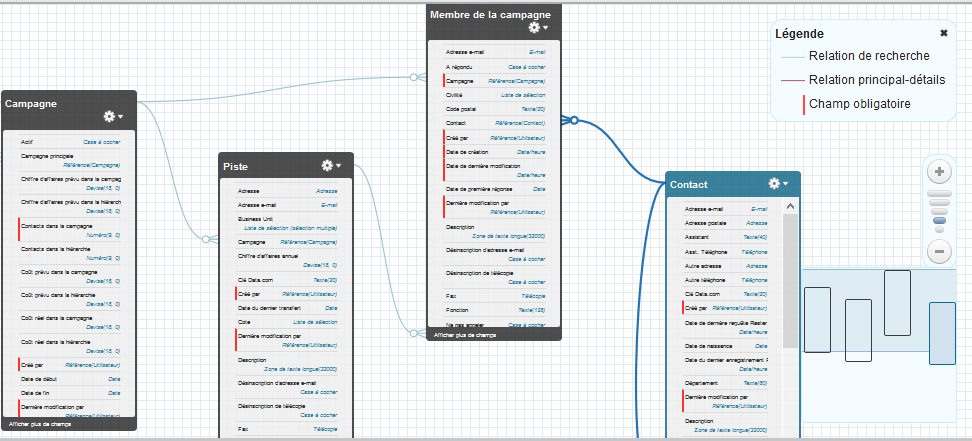
\includegraphics[scale=0.6]{classmarketing.PNG}
	\label{fig:le schéma des objets du processus de marketing}
\end{figure}

\subsection{développement et réalisation}
la plateforme Salseforce.com offre le service pour l'envoi en mass des email. mais la selection des destinataires posait un problème  vu qu'il n'y avait pas d'option pour le filtrage, pour celà nous avons commencer la création  d'une interface de selection des destinataires selon plusiuers filtres.
le processus de marketing ne s'arrête pas à l'envoi des mails mais nous avons besoin de recevoir les réponses des membres de la campagne.  pour celà nous avons suivi les étapes suivantes:
\begin{enumerate}
	\item Configure Email to SalesForce : cette étape se fait au niveau de la plateforme salesforce, cette option permet aux utilisateurs d'attribuer des courriels aux prospects, aux contacts, aux opportunités et à d'autres enregistrements spécifiques dans Salesforce. De cette façon, il est facile de suivre les communications liées aux ventes.
	
	\begin{figure}[H]
		\centering
			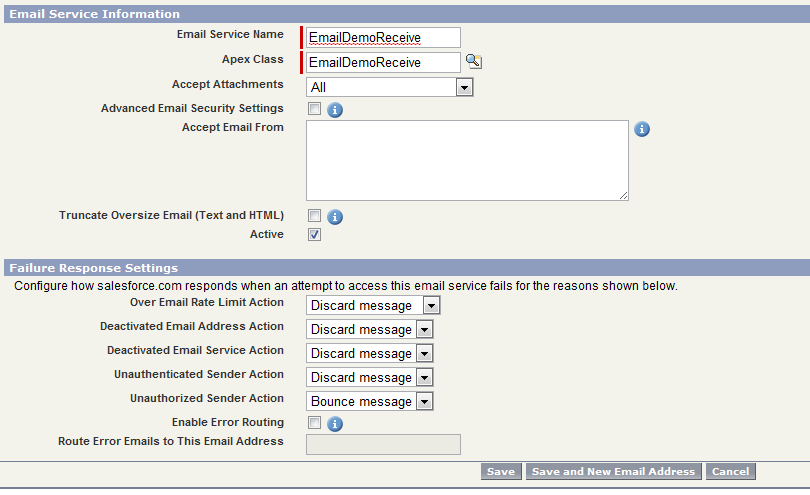
\includegraphics[scale=0.5]{Email_1.png}
		\label{fig:Configuration de "Email to SalesForce"}
	\end{figure}
	
	\item Configure BCC compliance (wide org BCC): cette fonctionnalité permet d'envoyer automatiquement une copie cachée de chaque message électronique sortant à une adresse email que nous avons spécifié.
	\item wide org Footer:  c'est un pied de page utilisé dans tous les message sortant de la plateforme , pour qu'il soit utilisé par la suite dans le script Google pour identifier les Mail venant de 		Salesforce
	\item Inbound Email handler: class Apex pour recevoir les réponses venants de Google, et enregistrer la réponse comme activité liée au contact ou piste ayant la même addresse mail que le message reçue.
	
	\begin{figure}[H]
		\centering
			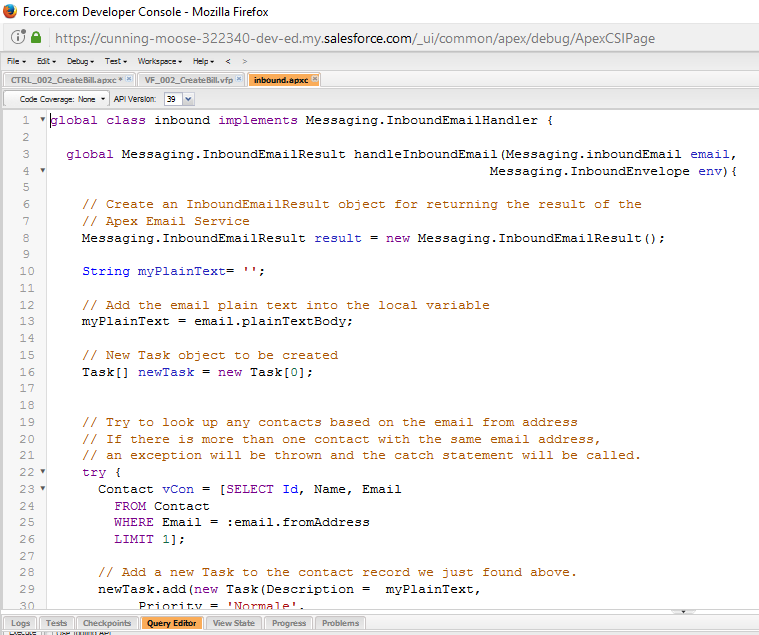
\includegraphics[scale=0.7]{inbound.PNG}
		\label{fig:inbound}
	\end{figure}
	
 
\item Script Google  : Google offre un service appelé GoogleScript permet de  scripter le language JS dans le cloud  et qui offre des moyens faciles d'automatiser les tâches sur les produits Google et des services tiers et de créer des applications Web. Dans notre cas il est utilisé pour identifier les message qui sont une réponse à un message venant de la plateforme salesforce et puis renvoyer la réponse à Salesforce.
\end{enumerate}
la figure suivante représente une portion du code Sur Google Script.
\begin{figure}[H]
	\centering
		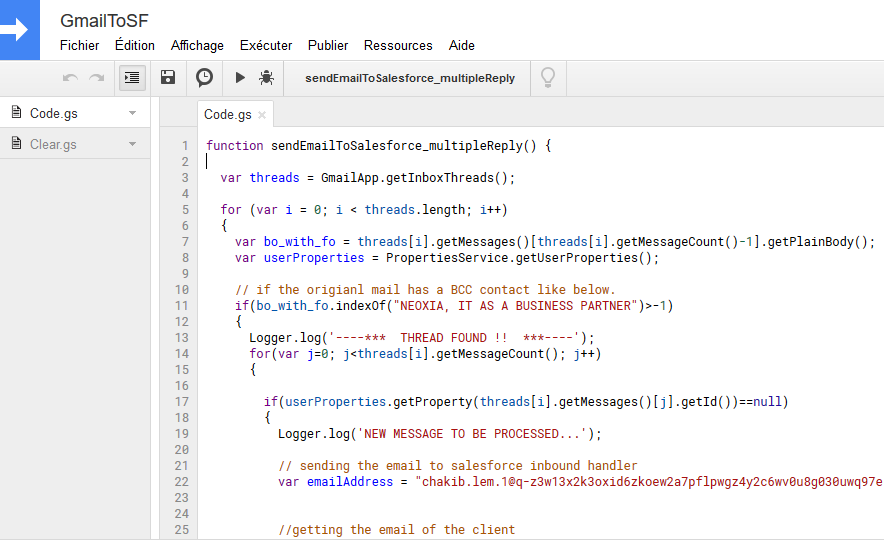
\includegraphics[scale=0.7]{googlescript.PNG}
	\label{fig:googlescript}
\end{figure}
le schéma montre l'inétarction entre les Systèmes GoogleScript, le Client, et SF:
\begin{figure}[H]
	\centering
		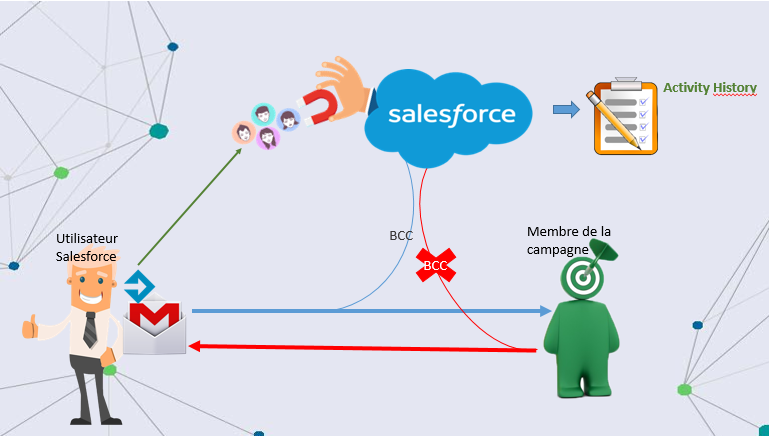
\includegraphics[scale=0.7]{EmailMarketing.PNG}
	\label{fig:EmailMarketing}
\end{figure}

\subsection {dificultés et limitations}
comme le client peut nous répondre à partir de plusieurs client messagerie, la capture de la réponse deviens difficile car chaque client a une structure de message différente 
pour celà nous nous avons contenter de l'analyse des réponses des deux clients : gmail et Outlook.
la figure ci-dessous montre la réception de la réponse et la tâche enregitrée.
\begin{figure}[H]
	\centering
		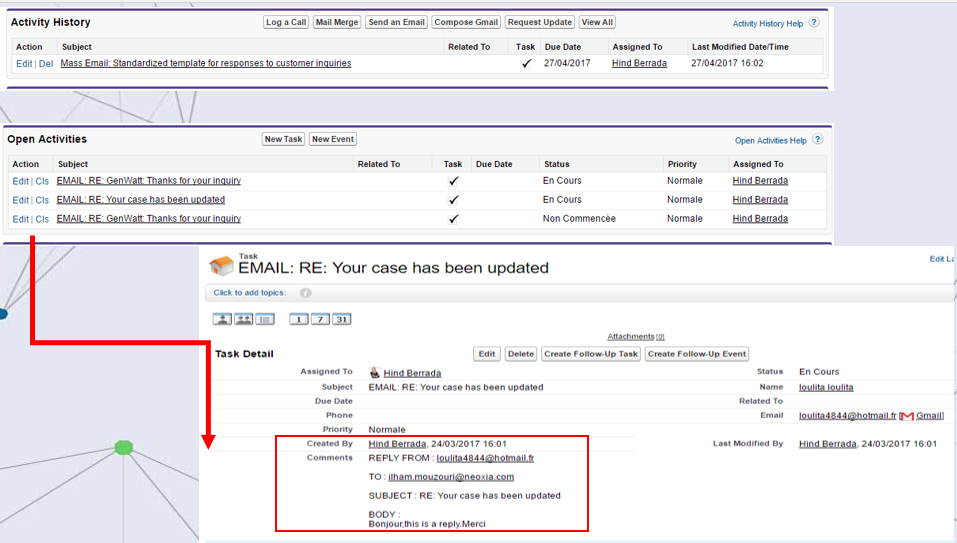
\includegraphics{reponsemail.PNG}
	\label{fig:Interface de la réception de la réponse par mail}
\end{figure}
\section {processus de Facturation}
\subsection{conception initiale}
Comme tout processus nous avons commencer par l'élaboration des Objets Standards et personnalisés pour gérer la facturation,
Facture, Echeance, Opportunité,Poste d'Opportunité, Poste d'echeance.
la figure ci-dessous montre les Objets principales et les relations entre eux.
\begin{figure}[H]
	\centering
		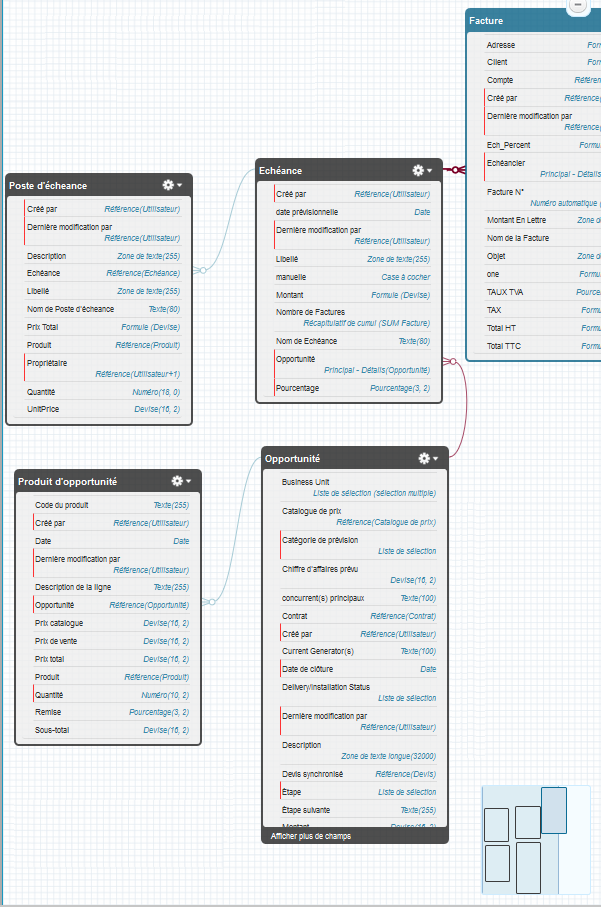
\includegraphics{classfacturation.PNG}
	\label{fig:classfacturation}
\end{figure}





\section{Etablissement des rapports et des tableau de bord}
\paragraph{}Le reporting constitue un outil décisionnel aussi bien pour la Direction Générale que pour les Directions Opérationnelles. Il centralise les informations clés susceptibles d'aider à faire le point sur une partie de l'activité de l'entreprise (marketing, commerciale, financière, ..) et puis de piloter le business de façon efficace. 
\paragraph{}
Dans cette solution, le reporting représente un moyen tangible de prise de décision puisqu'il permet de traiter toutes les informations de l'analyse d’une manière détaillée et facile à comprendre.
\paragraph{}
Dans ce but, nous avons utilisé le connecteur direct à Salesforce de Tableau, nous pouvons analyser toutes les étapes du processus de commercial. Mettons en œuvre des tableaux de bord autonomes et des fonctions analytiques avancées concernant la prospection, la gestion de la clientèle potentielle et des opportunités, l'étude de nos perspectives commerciales, la gestion de comptes et bien plus encore.
\paragraph{}
 Cet outil permet de présenter les informations commerciales sous formes de rapports, accessibles depuis le CRM Salesforce, qui contiennent des tableaux et des graphes assistant la compréhension des données et permettant d’en tirer des conclusions congruentes.
\paragrapg{}
Dans cette section, nous exposerons les rapports et les tableaux de bords qui vont nous aider à prendre les décisions afin d'améliorer notre rentabilité à long terme.
\subsubsection{les rapports}
\paragraph{}
Un rapport renvoie un ensemble d'enregistrements qui remplissent certains critères et les affiche dans des lignes et des colonnes organisées. Les données de rapport peuvent être filtrées, groupées et affichées dans un graphique. Les rapports sont stockés dans des dossiers qui en contrôlent l'accès. 


\paragraph{}
A la fin de ce chapitre, nous avons utilisé des rapports pour exploiter les données accumulées au fil du temps par le projet. Nous pouvons examiner les données de notre projet dans presque toutes les combinaisons, les afficher sous des formats conviviaux et les partager les enseignements des résultats via des tableaux de bord.
\begin{figure}[H]
	\centering
		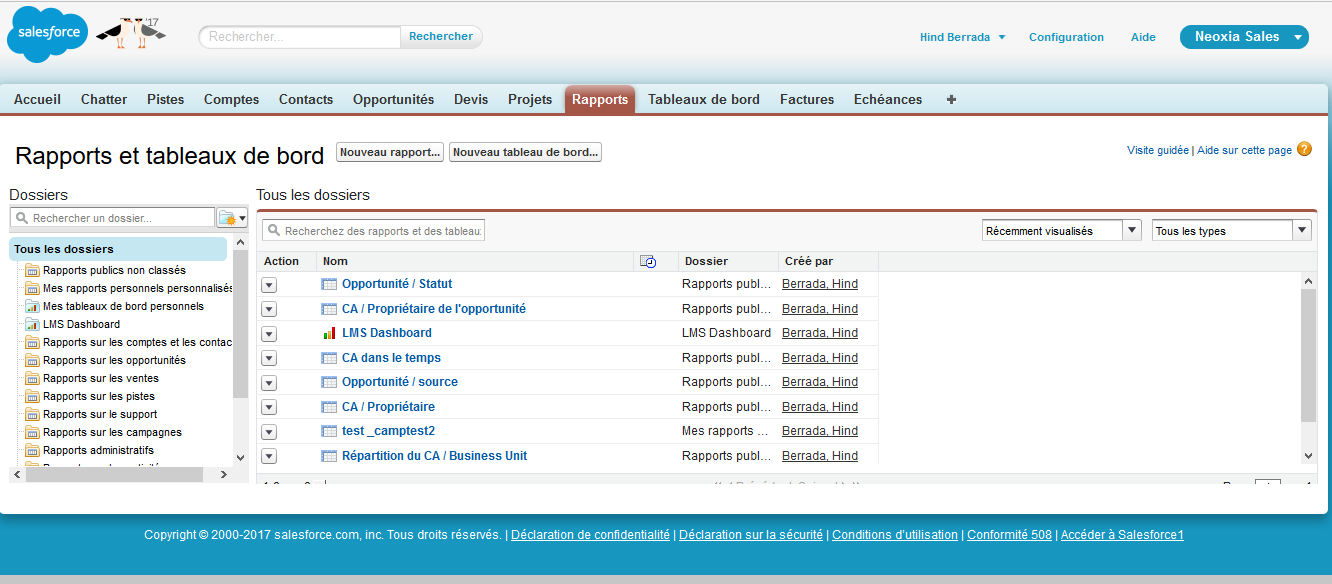
\includegraphics{rapportettb.PNG}
	\label{fig:Objet rapports}
\end{figure}
\paragraph{}
Pour notre projet Neoxia Sales, nous avons établi plusieurs rapports qui traduisent l'avancement du projet en prenant en considération plusieurs critères.
\paragraph{}
L'affichage des certains champs et non des autres se base sur des filtres à configurer selon les outputs que nous voudrions afficher sur nos rapports.
\begin{figure}[H]
	\centering
		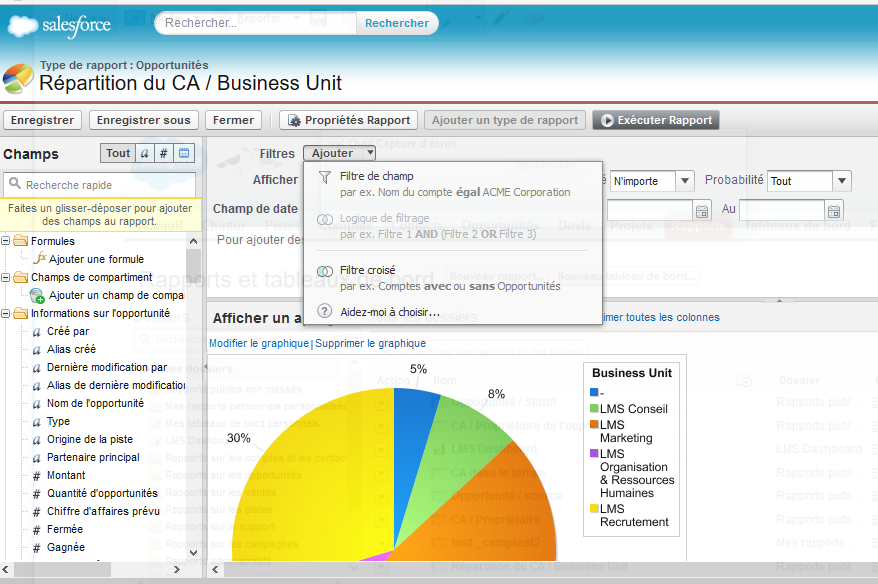
\includegraphics{rapportBU.PNG}
	\label{fig:Application des filtres sur le rapport}
\end{figure}
\paragraph{}
Ensuite, nous avons choisi le champ sur lequel nous voulons regrouper nos données ainsi les champs à afficher sur le rapport.
\paragraph{}
Les enregistrements s'affichent sur les rapports avec une vue claire.
\begin{figure}[H]
	\centering
		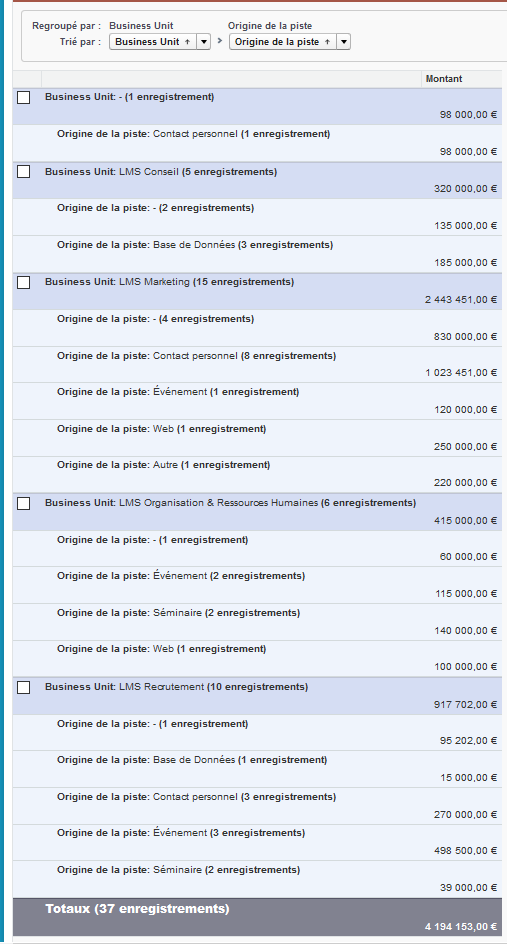
\includegraphics{resultatfiltrage.PNG}
	\label{fig:resultatfiltrage}
\end{figure}
\subsubsection{Les tableaux de bord:}
\paragraph{}
Une fois les données dont nous avons besoin rassemblées, nous utiliserons un tableau de bord pour rechercher des partenaires, rester en permanence informé(e) des changements, et partager des informations sur lesquelles nous et nos collaborateurs pouvons agir en temps réel
\paragraph{}
La première des choses c'est de choisir le type de composant et les sources de données qui sont nos rapports déjà exposés ci-avant

\begin{figure}[H]
	\centering
		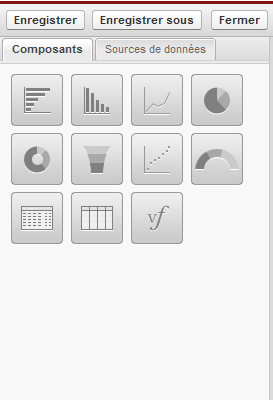
\includegraphics{composantsTB1.PNG}
	\label{fig:composantsTB1}
\end{figure}
\begin{figure}[H]
	\centering
		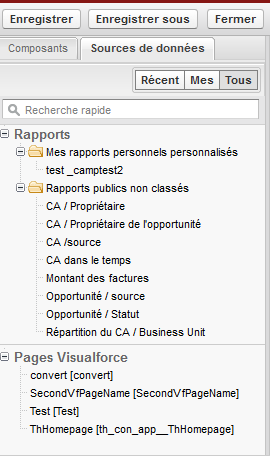
\includegraphics{composantsTB2.PNG}
	\label{fig:composantsTB1}
\end{figure}
\paragraph{}
Nous avons glissé, dans un premier temps, le composant sur lequel nous voulons travailler ensuite le rapport en question.
\begin{figure}[H]
	\centering
		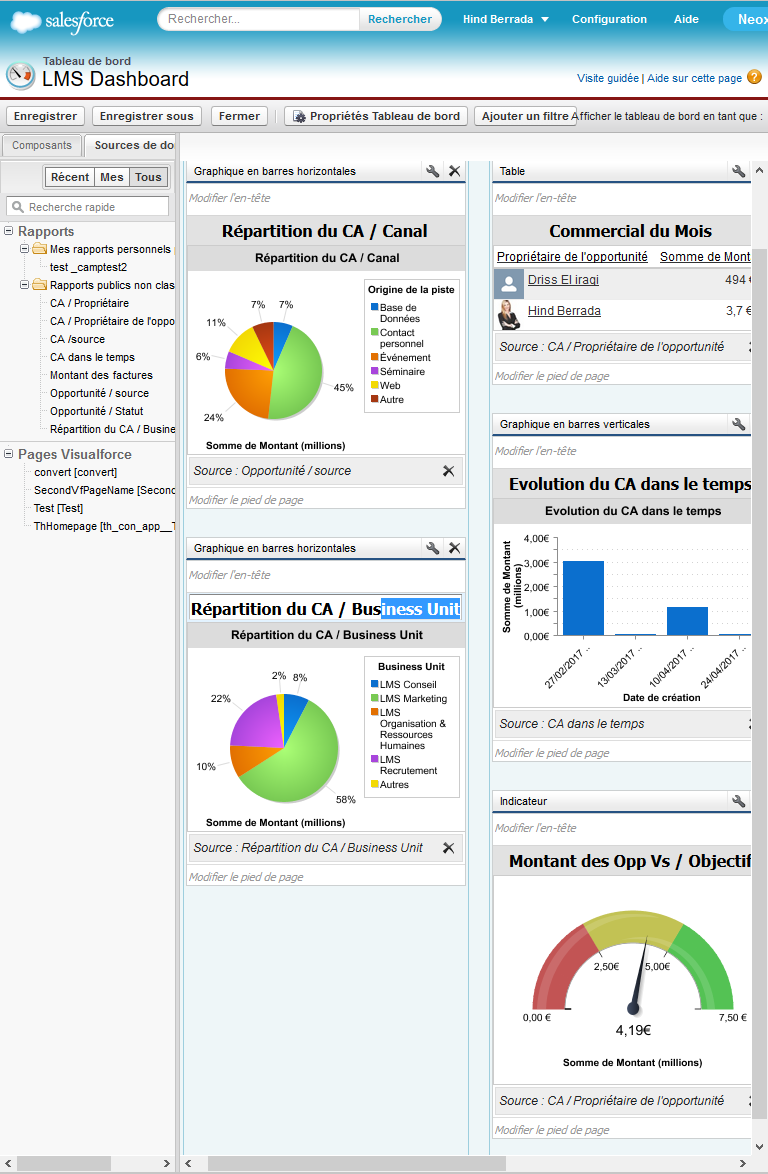
\includegraphics{dashbord.PNG}
	\label{fig:Exemples des tableaux de bord}
\end{figure}
\paragraph{}
Finalement, nous avons affiché nos tableaux de bord sur la page d'accueil. Aussi, nous pouvons personnaliser ces tableaux de bord selon nos besoins.
\begin{figure}[H]
	\centering
		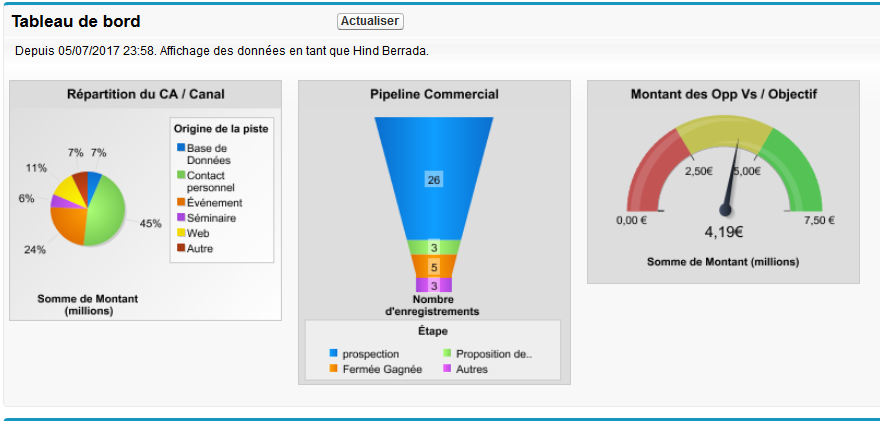
\includegraphics{rapports.PNG}
	\label{fig:rapports}
\end{figure}
 




% -_-_-_-_-_-_-_-_-_-_-_-_ FIN Realisation  -_-_-_-_-_-_-_-_-_-_-_-_

% -_-_-_-_-_-_-_-_-_-_-_-_ Conclusion  -_-_-_-_-_-_-_-_-_-_-_-_

\chapter*{\textsc{Conclusion}}
\addcontentsline{toc}{chapter}{\textsc{Conclusion}}

'\paragraph{}
Ce projet de fin d'études, effectué au sein de Neoxia MAROC, consiste en la réalisation d'une Solution CRM pour la gestion du processus commercial de Neoxia Maroc.
\paragraph{}
Durant ce stage, il a été convenu de suivre la méthodologie incrémentale itérative. La réalisation de ce projet requiert une bonne maîtrise des outils techniques ainsi qu'une bonne connaissance de la plate-forme de développement Force.com. Des formations métier, fonctionnelles et techniques ont donc été indispensables et ont été menées dans une période de préparation. 
\paragraph{}
La première itération du projet a consisté en la définition du périmètre du projet et l'étude de l'existant. Les itérations qui suivent ont été consacrées à la réalisation de plusieurs modules métier qui ont une grande valeur ajoutée pour les utilisateurs de la plateforme. Lors de chaque itération, une étude fonctionnelle a été effectuée suivie d'une étude technique si nécessaire. Enfin une conception détaillée est mise en place, pour pouvoir par la suite enchainer sur la phase de réalisation et de développement des modules en question.

 

% -_-_-_-_-_-_-_-_-_-_-_-_ FIN Conclusion  -_-_-_-_-_-_-_-_-_-_-_-_

% -_-_-_-_-_-_-_-_-_-_-_-_ Annexes  -_-_-_-_-_-_-_-_-_-_-_-_

% -_-_-_-_-_-_-_-_-_-_-_-_ FIN Annexes  -_-_-_-_-_-_-_-_-_-_-_-_

% -_-_-_-_-_-_-_-_-_-_-_-_ Références  -_-_-_-_-_-_-_-_-_-_-_-_

% -_-_-_-_-_-_-_-_-_-_-_-_ FIN Références  -_-_-_-_-_-_-_-_-_-_-_-_



\end{document}